


\documentclass[11pt,titlepage,twoside]{article}\usepackage[]{graphicx}\usepackage[table]{xcolor}
% maxwidth is the original width if it is less than linewidth
% otherwise use linewidth (to make sure the graphics do not exceed the margin)
\makeatletter
\def\maxwidth{ %
  \ifdim\Gin@nat@width>\linewidth
    \linewidth
  \else
    \Gin@nat@width
  \fi
}
\makeatother

\definecolor{fgcolor}{rgb}{0.345, 0.345, 0.345}
\newcommand{\hlnum}[1]{\textcolor[rgb]{0.686,0.059,0.569}{#1}}%
\newcommand{\hlsng}[1]{\textcolor[rgb]{0.192,0.494,0.8}{#1}}%
\newcommand{\hlcom}[1]{\textcolor[rgb]{0.678,0.584,0.686}{\textit{#1}}}%
\newcommand{\hlopt}[1]{\textcolor[rgb]{0,0,0}{#1}}%
\newcommand{\hldef}[1]{\textcolor[rgb]{0.345,0.345,0.345}{#1}}%
\newcommand{\hlkwa}[1]{\textcolor[rgb]{0.161,0.373,0.58}{\textbf{#1}}}%
\newcommand{\hlkwb}[1]{\textcolor[rgb]{0.69,0.353,0.396}{#1}}%
\newcommand{\hlkwc}[1]{\textcolor[rgb]{0.333,0.667,0.333}{#1}}%
\newcommand{\hlkwd}[1]{\textcolor[rgb]{0.737,0.353,0.396}{\textbf{#1}}}%
\let\hlipl\hlkwb

\usepackage{framed}
\makeatletter
\newenvironment{kframe}{%
 \def\at@end@of@kframe{}%
 \ifinner\ifhmode%
  \def\at@end@of@kframe{\end{minipage}}%
  \begin{minipage}{\columnwidth}%
 \fi\fi%
 \def\FrameCommand##1{\hskip\@totalleftmargin \hskip-\fboxsep
 \colorbox{shadecolor}{##1}\hskip-\fboxsep
     % There is no \\@totalrightmargin, so:
     \hskip-\linewidth \hskip-\@totalleftmargin \hskip\columnwidth}%
 \MakeFramed {\advance\hsize-\width
   \@totalleftmargin\z@ \linewidth\hsize
   \@setminipage}}%
 {\par\unskip\endMakeFramed%
 \at@end@of@kframe}
\makeatother

\definecolor{shadecolor}{rgb}{.97, .97, .97}
\definecolor{messagecolor}{rgb}{0, 0, 0}
\definecolor{warningcolor}{rgb}{1, 0, 1}
\definecolor{errorcolor}{rgb}{1, 0, 0}
\newenvironment{knitrout}{}{} % an empty environment to be redefined in TeX

\usepackage{alltt}
\usepackage[a4paper, inner=1.5cm, outer=1.5cm, top=2cm, bottom=3cm]{geometry}

\usepackage[utf8]{inputenc} 
\usepackage[T1]{fontenc}
\usepackage[sort&compress]{natbib}
\usepackage[french]{babel}

\addto\captionsfrench{\def\tablename{Tableau}}
\addto\captionsfrench{\renewcommand*{\contentsname}{Sommaire:}}
\addto\captionsfrench{%
  \renewcommand{\listfigurename}{Liste des figures:}%
  \renewcommand{\listtablename}{Liste des tableaux:}%
  \renewcommand{\abstractname}{Résumé}%
}
\usepackage{caption}
\usepackage[labelsep=endash]{caption}
\usepackage{graphicx}
\usepackage{colortbl}
\usepackage{booktabs}
\usepackage{longtable}
\usepackage{array}
\usepackage{multirow}
\usepackage{wrapfig}
\usepackage{float}
\usepackage{pdflscape}
\usepackage{tabu}
\usepackage{threeparttable}
\usepackage{threeparttablex}
\usepackage[normalem]{ulem}
\usepackage{makecell}
\usepackage[table]{xcolor}
\usepackage{ae,aeguill}
\usepackage{subcaption}

\usepackage{authblk}
\renewcommand\Authand{ et }
\renewcommand\Authands{ et }

\usepackage{textcomp}
\usepackage{hyperref}
\pdfstringdefDisableCommands{%
  \def\\{}%
  }
\hypersetup{ 
colorlinks=true, 
linkcolor=blue, 
citecolor=blue, 
filecolor=blue, 
urlcolor=blue, 
pdftitle= {Suivi des poissons migrateurs sur les STACOMI du bassin de la Seine\\ Année 2023 }, pdfauthor={Sébastien Grall},
pdfsubject={stacomi},
 pdfkeywords={stacomi} {migrateurs} {Seine} {poissons}
}
\pdfoptionpdfminorversion=7
\renewcommand{\sectionmark}[1]{\markboth{}{\emph{\thesection~#1}}}
\renewcommand{\subsectionmark}[1]{\markboth{}{\emph{\thesubsection~#1}}}
\renewcommand{\subsubsectionmark}[1]{\markboth{}{\emph{\thesubsection~#1}}}

\makeatletter
    \def\@@and{et}
\makeatother

\usepackage{fancyhdr}
\pagestyle{fancy}
\fancyhf{}
\rhead{\rightmark}
\lfoot{\footnotesize{Suivi des poissons migrateurs sur les STACOMI du bassin de la Seine, année 2023}} %Insere un pied de page avec le texte a gauche.
\rfoot{\thepage}
\setlength{\headheight}{15pt}

\usepackage{pdfpages}
\usepackage{setspace}

%%%%%%%%%%%%%%%%%%%%%%%%%%%%%%%%%%%%%%%%%%%
%%%%%% CHUNK DE CHARGEMENT INITIAL  %%%%%%%
%%%%%%%%%%%%%%%%%%%%%%%%%%%%%%%%%%%%%%%%%%%


%% Makes a path to your graphics' folder.
\graphicspath{{image/}}

\title{Suivi des poissons migrateurs sur les STACOMI du bassin de la Seine,
année 2023}

\author[1]{Sébastien Grall}
\author[1]{Alice Lemonnier}
\author[1]{Romain Dupuy-Jandard}
\author[2]{Mathilde Castro}
\affil[1]{Seine-Normandie Migrateurs, 11 cours Clemenceau 76100 Rouen}
\affil[2]{Fédération Départementale de l’Oise pour la Pêche et la protection des Milieux Aquatiques, 28 rue Jules Méline 60200 Compiègne}
\IfFileExists{upquote.sty}{\usepackage{upquote}}{}
\begin{document}

\hypersetup{pageanchor=false}

\begin{titlepage}

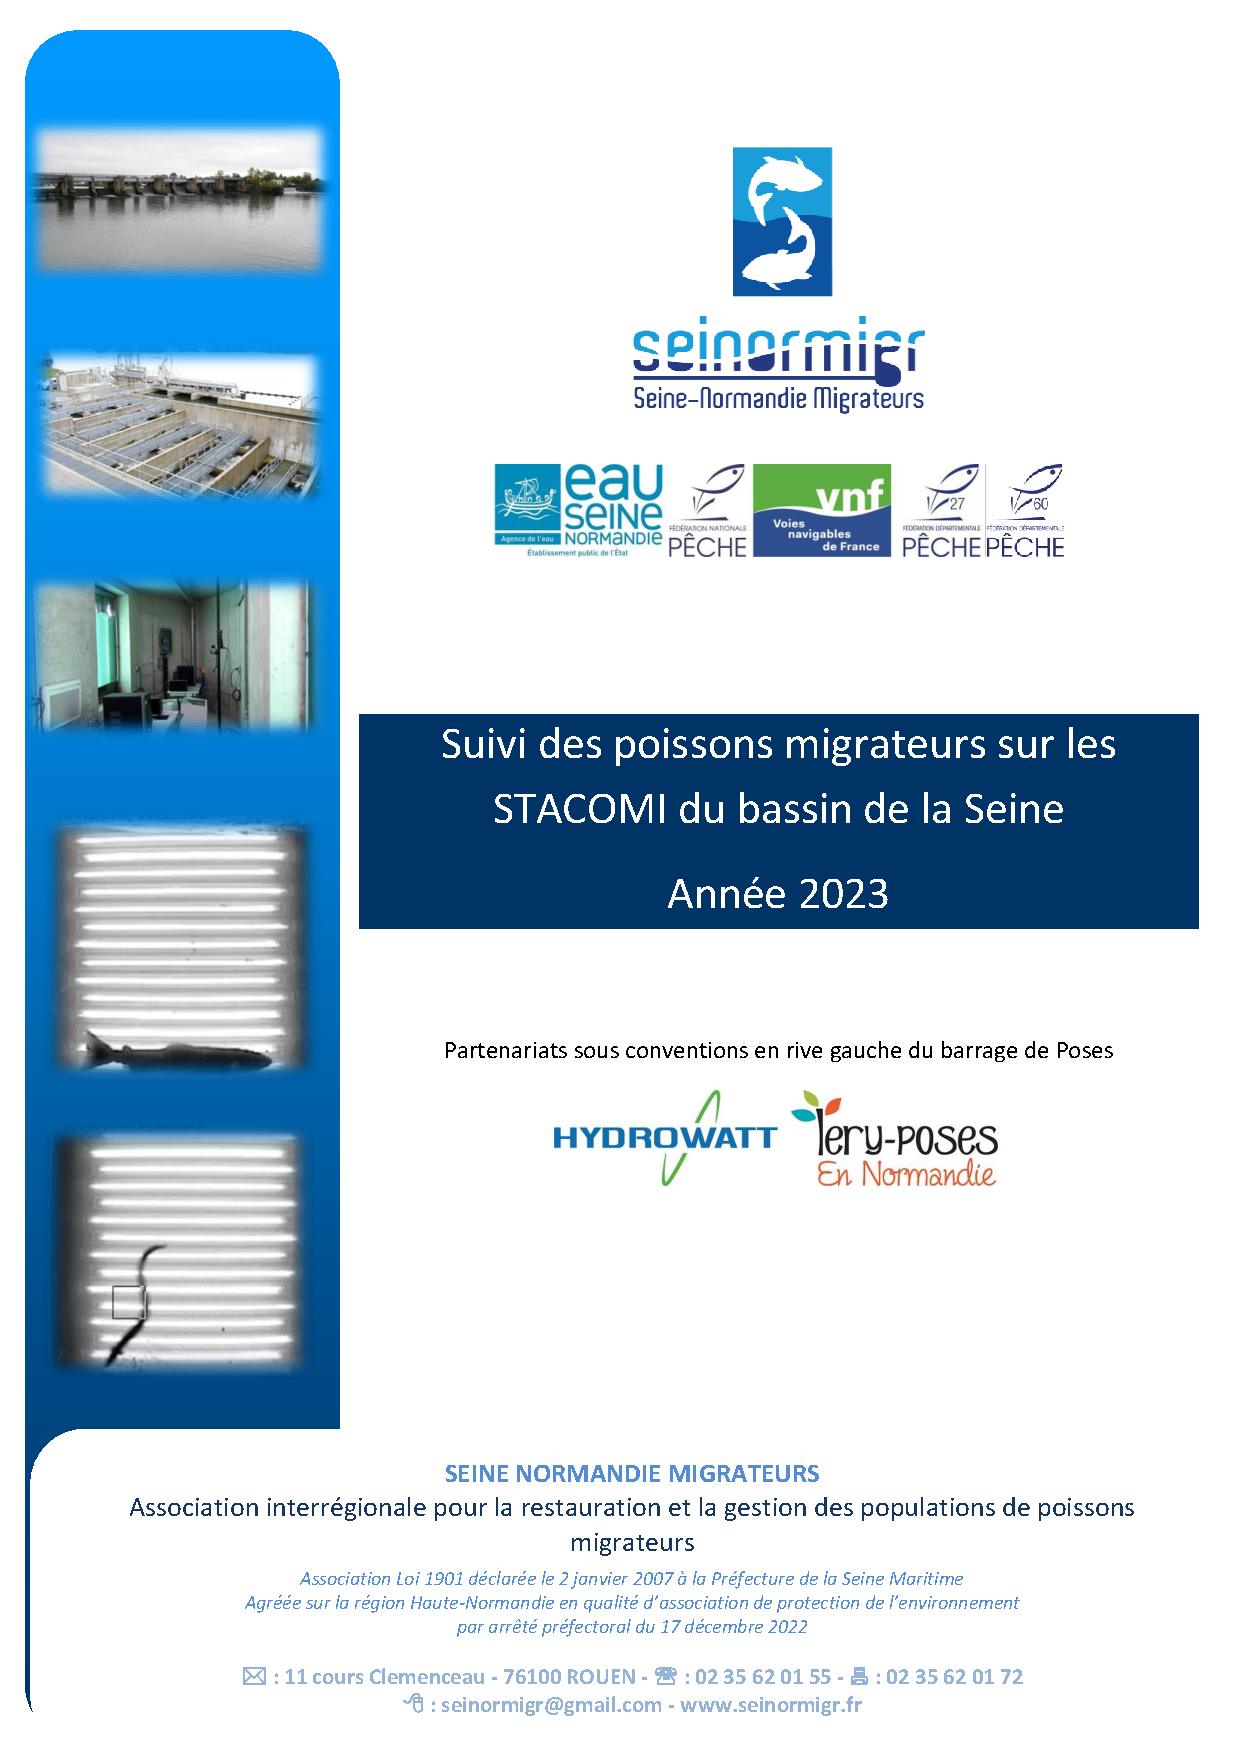
\includepdf[pages=-]{frontpage.pdf}

\end{titlepage}


\newpage
\thispagestyle{empty}
\strut
\newpage

\pagenumbering{roman} \setcounter{page}{1}

\maketitle

\begin{abstract}

Le résumé

\end{abstract}

\newpage

\tableofcontents

\clearpage

\listoffigures

\listoftables

\hypersetup{pageanchor=false}

\clearpage

\pagenumbering{arabic} \setcounter{page}{1} 

\section{Introduction}

La situation de l'ensemble des poissons migrateurs dans le monde
est similaire : le nombre de populations,
les aires de répartition et les abondances sont en déclin depuis la fin du 19\up{ème} siècle
\citep{saunders_atlantic_1981,bagliniere_reintroductions_1990,parrish_why_2011,jonsson_extinction_1999,
keith_atlas_2001,rochard_identification_2007,limburg_dramatic_2009}.
Le besoin de ces espèces de migrer entre différents habitats essentiels à la finalisation
de leur cycle biologique, implique une vulnérabilité particulière aux perturbations de l'environnement.
Aujourd'hui, la majorité des poissons amphihalins figure dans la liste rouge
des espèces menacées de l'IUCN \citep{limburg_dramatic_2009}.

Sur la Seine, le constat est analogue. Historiquement, 10 espèces amphihalines, dont 8 poissons grands migrateurs
fréquentaient le fleuve sur presque l'ensemble de son bassin versant \citep{moreau_histoire_1881,moreau_les_1898,
poplin_peuplement_1952,euzenat_migren_1992,rochard_identification_2007}, souvent en abondance. Cependant,
en raison d'une anthropisation toujours croissante du fleuve, c'est dès les années 1850 que le déclin s'est amorcé.
Les dégradations sont multiples et semblables à ce qui a été démontré sur d'autres systèmes fluviaux
\citep{nehlsen_pacific_2011,mcdowall_different_1999,lichatowich_depletion_1999,mckinnell_spatial_1999,
limburg_dramatic_2009}. L'édification de barrages, la chenalisation, la pollution, la dégradation des habitats et la surpêche ont conduit au cours du 20\up{ème} siècle à l'extinction des derniers grands migrateurs
\citep{euzenat_migren_1992,belliard_peuplement_1994,mouchel_bassin_1998,boet_multiple_1999,rochard_identification_2007},
seule l'Anguille européenne subsistait encore \citep{boet_multiple_1999,rochard_identification_2007}.

Néanmoins, les efforts entrepris dans le traitement des effluents anthropiques, notamment ceux de l'agglomération parisienne, durant ces deux dernières décennies ont contribué à la franche amélioration de la qualité de l'eau de la Seine \citep{billen_programme_1999,belliard_return_2009,
gousailles_limpact_2009}. Ceci s'est rapidement traduit par le retour des poissons amphihalins, parmi lesquelles deux espèces estuariennes, l'Eperlan (\textit{Osmerus eperlanus}) \citep{pomfret_spatial_1991} et le Flet commun
(\textit{Platichthys flesus}); mais notamment 6 espèces appartenant à la communauté historique des grands poissons
migrateurs de la Seine \citep{rochard_identification_2009} telles que le Saumon atlantique (\textit{Salmo salar}),
la Truite de mer (\textit{Salmo trutta trutta}), la Grande alose (\textit{Alosa alosa}), l'Alose feinte
(\textit{Alosa fallax}) \citep{duhamel_peuplement_2004}, la Lamproie marine (\textit{Petromyzon marinus}) et la
Lamproie fluviatile (\textit{Lampetra fluviatilis}), qui recolonisent peu à peu les parties les plus basses du bassin. L'Anguille européenne (\textit{Anguilla anguilla}) est, quant à elle, présente également sur les zones amonts bien que ses effectifs soient relictuels.

Dès lors, il s'est rapidement avéré primordial de suivre l'évolution de la recolonisation de ces espèces. Pour ce faire, il s'agit de s'intéresser aux éléments clés du cycle biologique liés au domaine continental chaque année. Cela implique
le recensement des zones de frayères et du succès reproducteur; mais avant tout, le dénombrement des géniteurs en montaison en différents points du bassin versant en réponse notamment aux travaux de restauration de la continuité écologique sur le fleuve.

C'est au barrage de Poses dans l'Eure (27), le premier ouvrage sur l'axe Seine, que se sont organisés les premiers éléments de ce suivi, avec la mise en place d'une Station de Contrôle des Migrations (STACOMI) sur la passe à poissons existante en rive gauche depuis octobre 2007. Afin d'assurer la mise en conformité de l'ouvrage dans le cadre du plan de gestion Anguille, le dispositif a été complété en 2013 par l'ajout d'une passe piège à anguilles sur cette même rive.

En raison de la longueur de l'ouvrage (470m) et de la localisation sur le bassin, la rive droite a également été aménagée par les Voies Navigables de France (VNF). Ce nouveau dispositif, mis en service à l'automne 2017 est constitué d'une passe à bassins équipée d'une chambre de vidéo-comptage ainsi qu'une passe piège à anguilles. A la même période une autre installation à vue le jour sur le barrage de Carandeau, première ouvrage sur l'Aisne. Depuis avril 2023, le barrage de Pontoise, première ouvrage sur l'Oise a également été équipé d'un système de vidéo-comptage.

Ce rapport présente les résultats des suivis sur les dispositifs de ,comptage des 3 ouvrages cités précédemment et les associent avec les données historiques afin de donner une vision globale de l'activité migratoire sur le bassin de la Seine.

\clearpage

\section{Contexte de l'étude}

\subsection{Le bassin de la Seine}

Longue de 776 km, la Seine prend sa source à Saint-Germain-Source-Seine en Côte d'Or (21) à 446 mètres d'altitude, pour se jeter dans la Manche au niveau du Havre (Figure \ref{reseau_stacomi}). Elle draine une surface de 78 650 km$^2$ représentant 14\% du territoire français. Ses principaux affluents sont l'Aube, l'Yonne, la Marne, l'Oise, l'Eure et la Risle.

\begin{figure}[htpb]
\centering
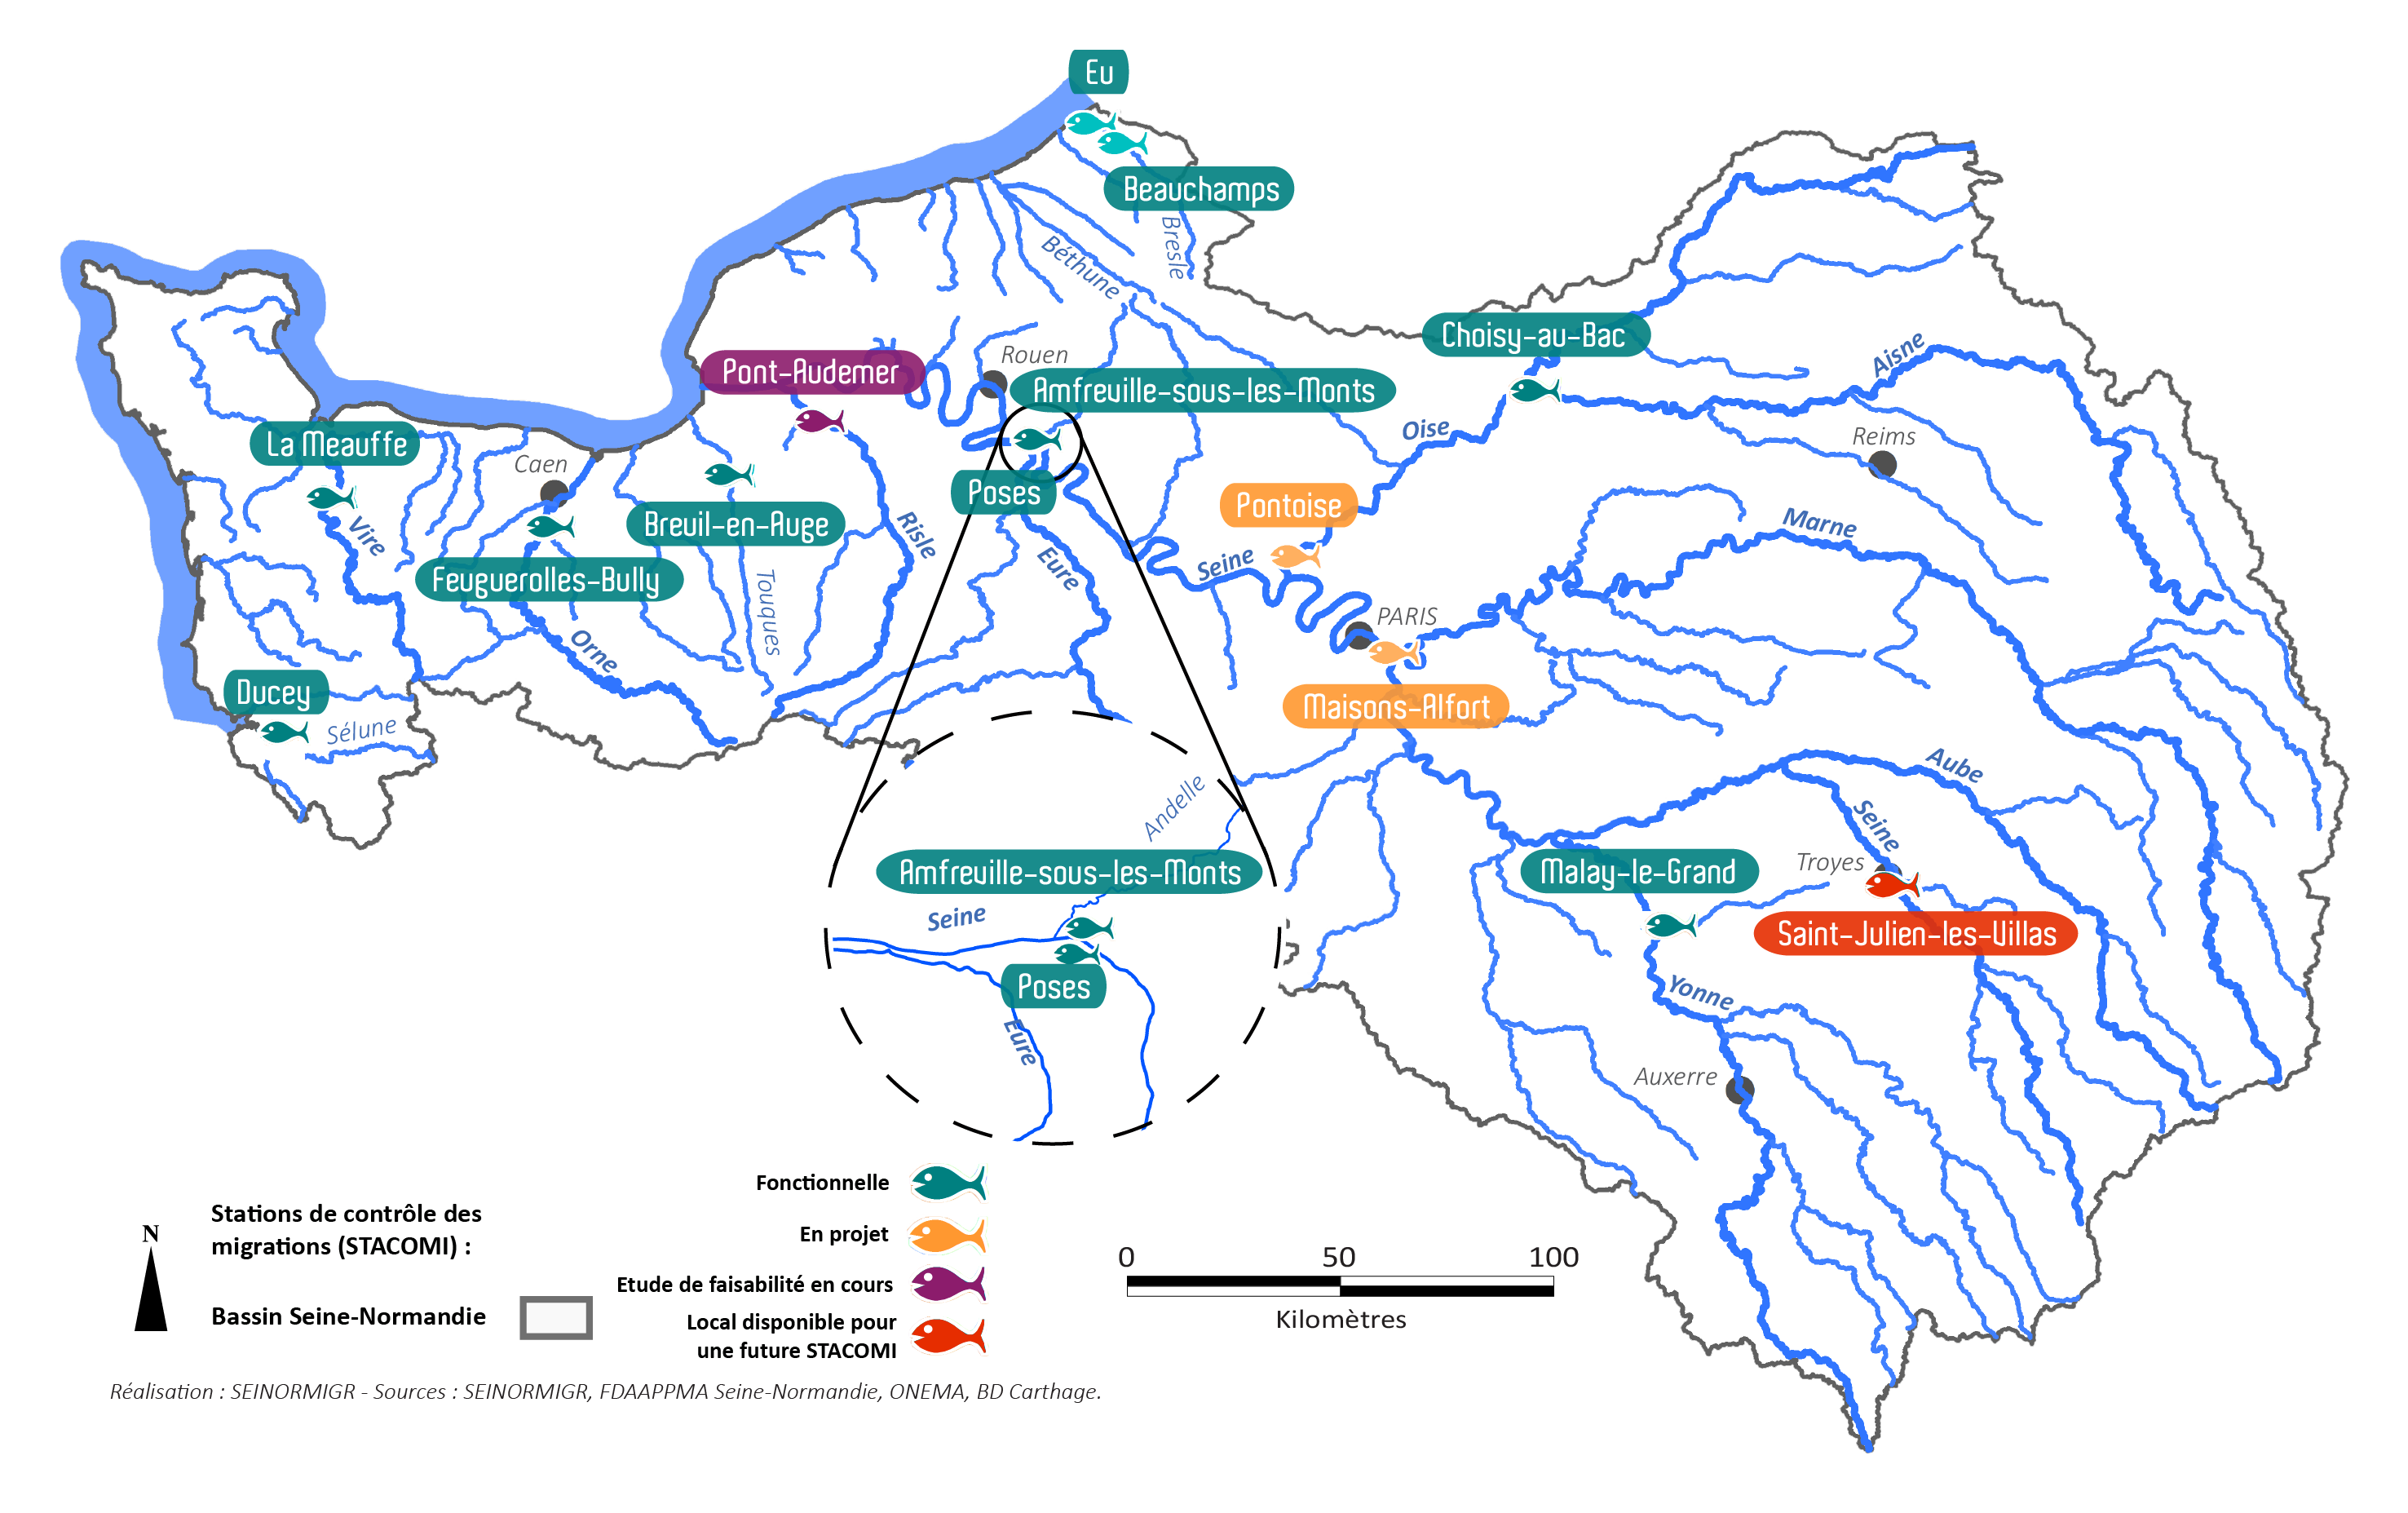
\includegraphics[width=\textwidth]{reseau_stacomi.png}
\caption{Le bassin Seine-Normandie, ses principaux cours d'eau et les stations de contrôle des migrations (STACOMI)}
\label{reseau_stacomi}
\end{figure}

En fond d'estuaire, le débit moyen du fleuve fluctue, ces dernières années, autour de 480m$^3$/s. En raison de la chenalisation et des ouvrages de gestion des crues, les variations hydrologiques de la Seine restent de nos jours relativement modérées, avec une élévation des niveaux d'eau récurrente au cours de la période hivernale
(Figure \ref{debit_seine_histo}).

\begin{figure}[htpb]
\centering
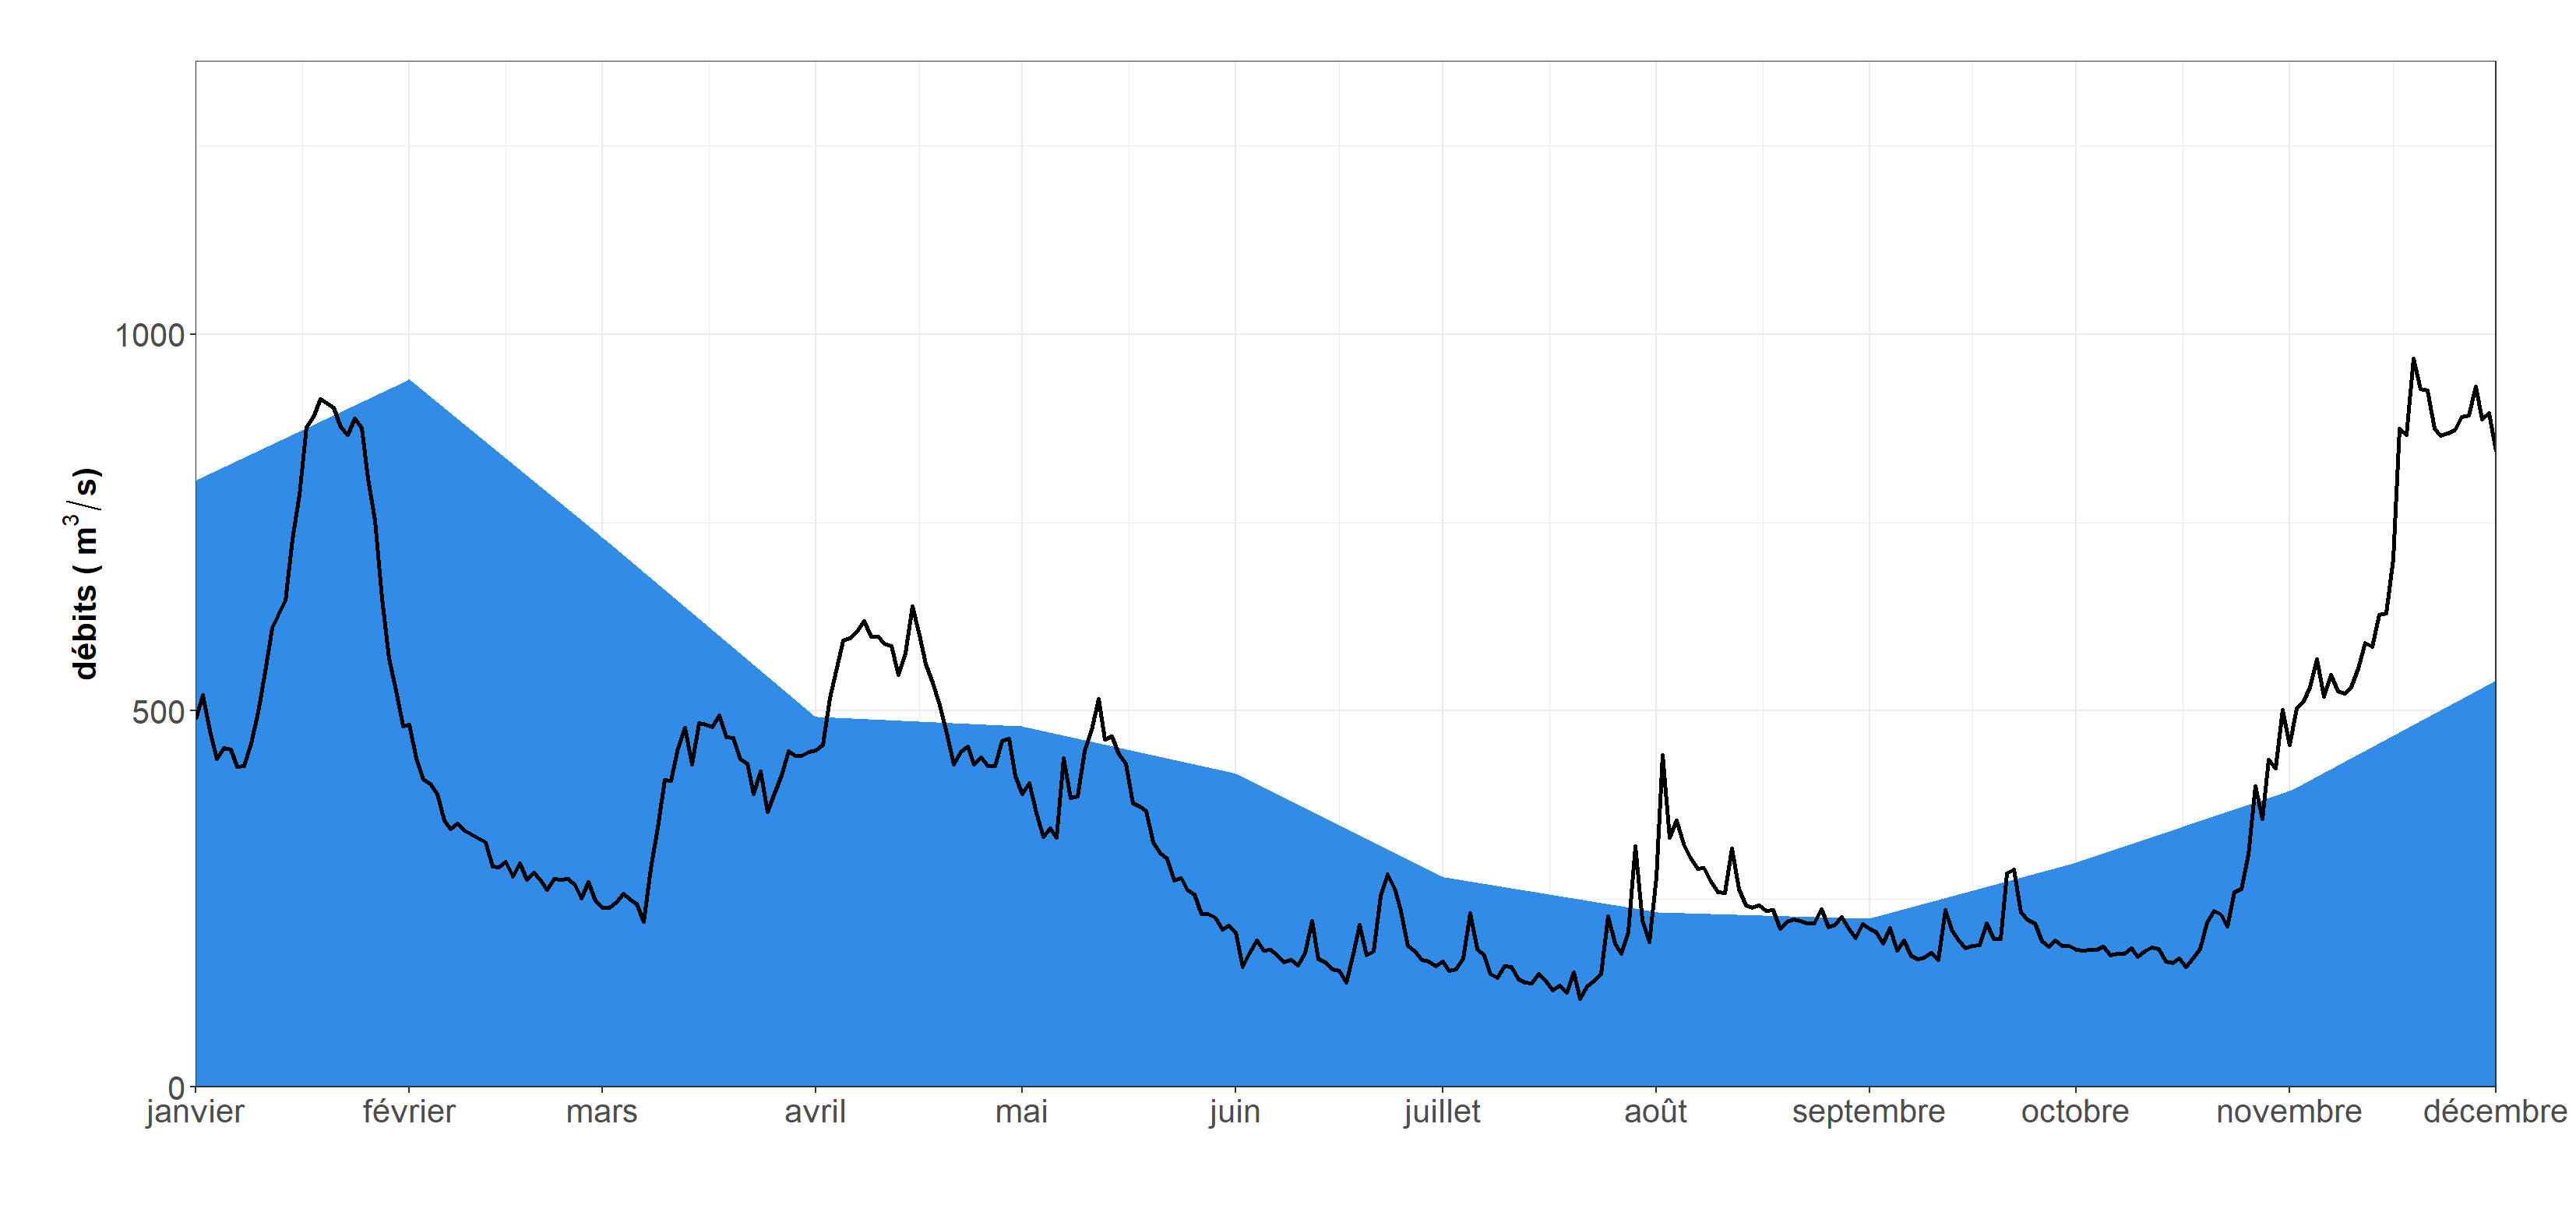
\includegraphics[width=0.8\textwidth]{debit_seine_histo.png}
\caption{Régime hydrologique de la Seine à Vernon, la moyenne interannuelle des dix années précédentes (2012 à 2022) est représentée en bleu, les débits journaliers de l'année sont présentés en noir}
\label{debit_seine_histo}
\end{figure}

Le réseau hydrographique de la Seine parcourt en tête de bassin quelques massifs cristallins et métamorphiques dans les Ardennes et le Morvan; mais s'étend principalement dans la cuvette sédimentaire qu'est le bassin parisien traversant des terrains à dominante calcaire, argileuse ou marneuse. Ce réseau présente les deux extrêmes en matière de densité de cours d'eau, avec des zones fortement densifiées sur les massifs anciens comme dans la Nièvre (58), et des zones crayeuses au drainage peu dense, mais avec un écoulement soutenu et régulier comme en Haute-Normandie.

La Seine est depuis plusieurs siècles une voie importante de communication et de commerce. Elle présente aujourd'hui 1 427 km de voies navigables, dont 496 km adaptées aux grands gabarits. C'est 50\% du trafic national qui y transite, avec Paris qui est le 1\up{er} port fluvial de France et le 2\up{ème} en Europe.

Plus de 18 millions de personnes habitent sur le bassin versant, correspondant à 27\% de la population nationale, dont 65\% (11,8 millions) dans la seule région d’Île de France. La Seine est considérée comme le fleuve le plus anthropisé de France. Les impacts physico-chimiques (détergents, pesticides...) et morphologiques (artificialisation des berges, chenalisation, édifications d'ouvrages...) se ressentent aujourd'hui dans tous les compartiments de l'écosystème, de la source à l'estuaire, jusqu'en baie de Seine.

\subsection{Situation des poissons grands migrateurs sur la Seine}

La Seine et ses affluents furent démunis de tous poissons migrateurs, exception faite de l'anguille, pendant plus de 80 ans. Cependant l'application d'un ensemble de mesures de conservation sur les habitats et les espèces, combinée à l'amélioration de la qualité de l'eau via le traitement des effluents ces deux dernières décennies, ont contribué aujourd'hui au retour de presque toutes les espèces migratrices. Les effectifs sont encore modestes par rapport aux populations pristines mais les différents travaux de restauration entrepris ont permis de faire entrer l'hydrosystème de la Seine dans une phase de recolonisation progressive. 

Les enjeux autour de la conservation des poissons grands migrateurs sont multiples. Ces espèces, de par leur biologie particulière, constituent un patrimoine écologique remarquable. Ces mêmes exigences biologiques et écologiques impliquent une certaine vulnérabilité aux perturbations de l'environnement, à tel point que la majorité des populations sont aujourd'hui menacées.

C'est par ailleurs logiquement que cette fragilité font des poissons migrateurs un indicateur pertinent de la qualité des milieux qu'ils fréquentent. Leur présence rend compte du bon fonctionnement et du bon état des écosystèmes aquatiques. L'image des migrateurs est d'ailleurs souvent associée à la restauration \og réussie \fg{} des cours d'eau, constituant par conséquent un bon support d'éducation à l'environnement.

De plus, ces espèces représentent une ressource économique importante pour la pêche professionnelle et/ou amateur. L'Union Européenne a montré par exemple que l'exploitation de l'Anguille européenne générait un revenu annuel de l'ordre de 183 millions d'euros.

Les mesures de conservation et de gestion s'appuient sur la connaissance des populations en place. C'est pourquoi, afin de permettre une recolonisation pérenne des espèces de poissons grands migrateurs dans ce système fluvial, il est indispensable de suivre son évolution. Pour ce faire, il s'agit de s'intéresser aux éléments clés liés aux phases du cycle biologique propres au domaine continental chaque année. Il est donc nécessaire de pouvoir estimer les effectifs migrants en différents points du bassin; de recenser les frayères actives, et d'évaluer le succès reproducteur, comme le fait annuellement la Fédération Départementale des Associations Agréées de Pêche et de Protection des Milieux Aquatiques de l'Eure (FDAAPPMA 27) pour la Lamproie marine sur la Basse-Andelle, l'Eure et l'Epte \citep{sanson_suivi_2009,sanson_suivi_2010,barault_suivi_2013,sanson_suivi_2013}(Figure \ref{photo_lamproies}); et dans l'ensemble d'identifier les zones recolonisées afin de situer les fronts de colonisation sur chacun des axes de migration. Les affluents de la Seine estuarienne (la Risle, l'Eure, l'Austreberthe, l'Andelle...) ont notamment un rôle particulier puisque leur proximité immédiate (malgré leur faible linéaire accessible) a permis de maintenir une population de poissons grands migrateurs sur le bassin et c'est certainement les générations issues de ces populations qui recolonisent le bassin versant.

\begin{figure}[hptb]
    \centering
    \begin{subfigure}[b]{0.45\textwidth}
        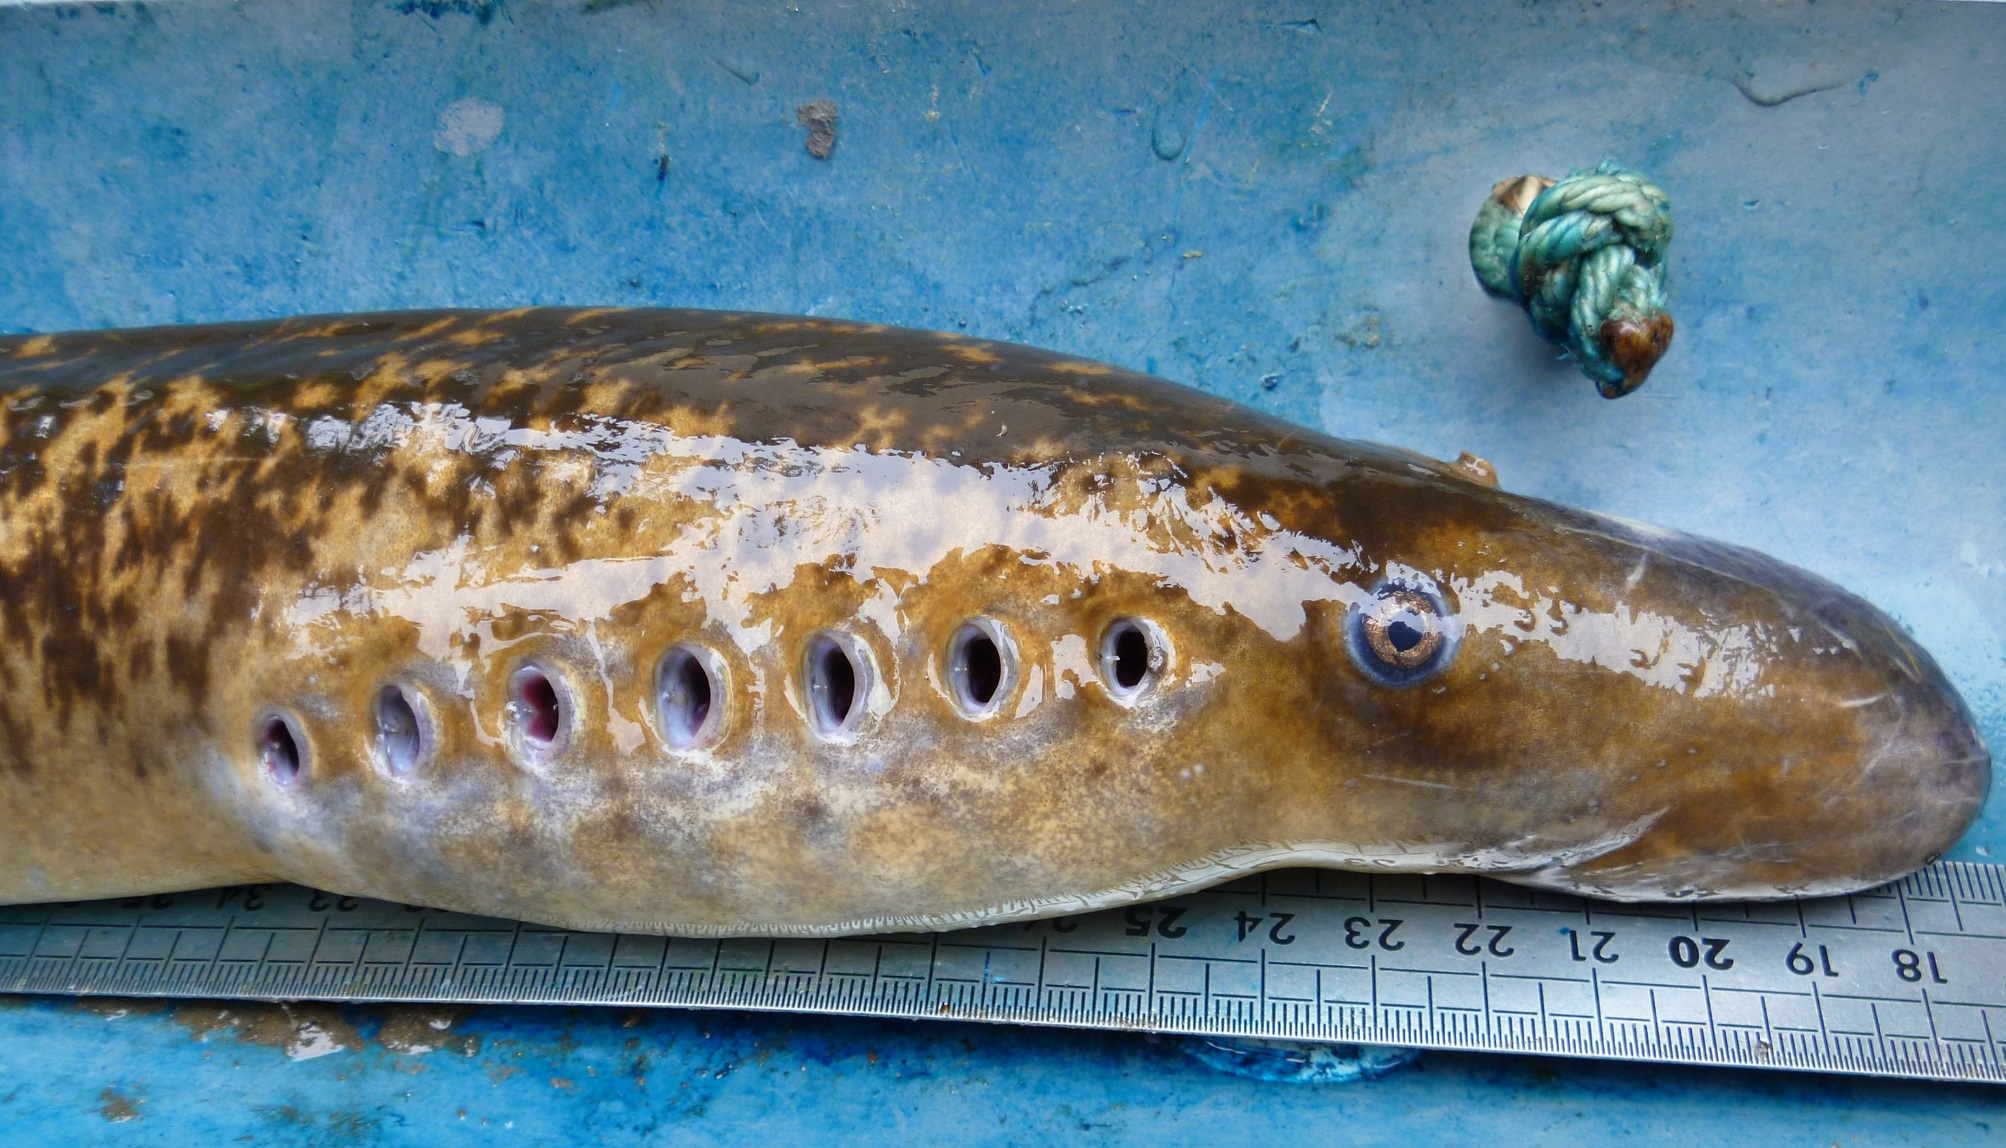
\includegraphics[width=\textwidth]{LPM_tete}
    \end{subfigure}
    \begin{subfigure}[b]{0.45\textwidth}
        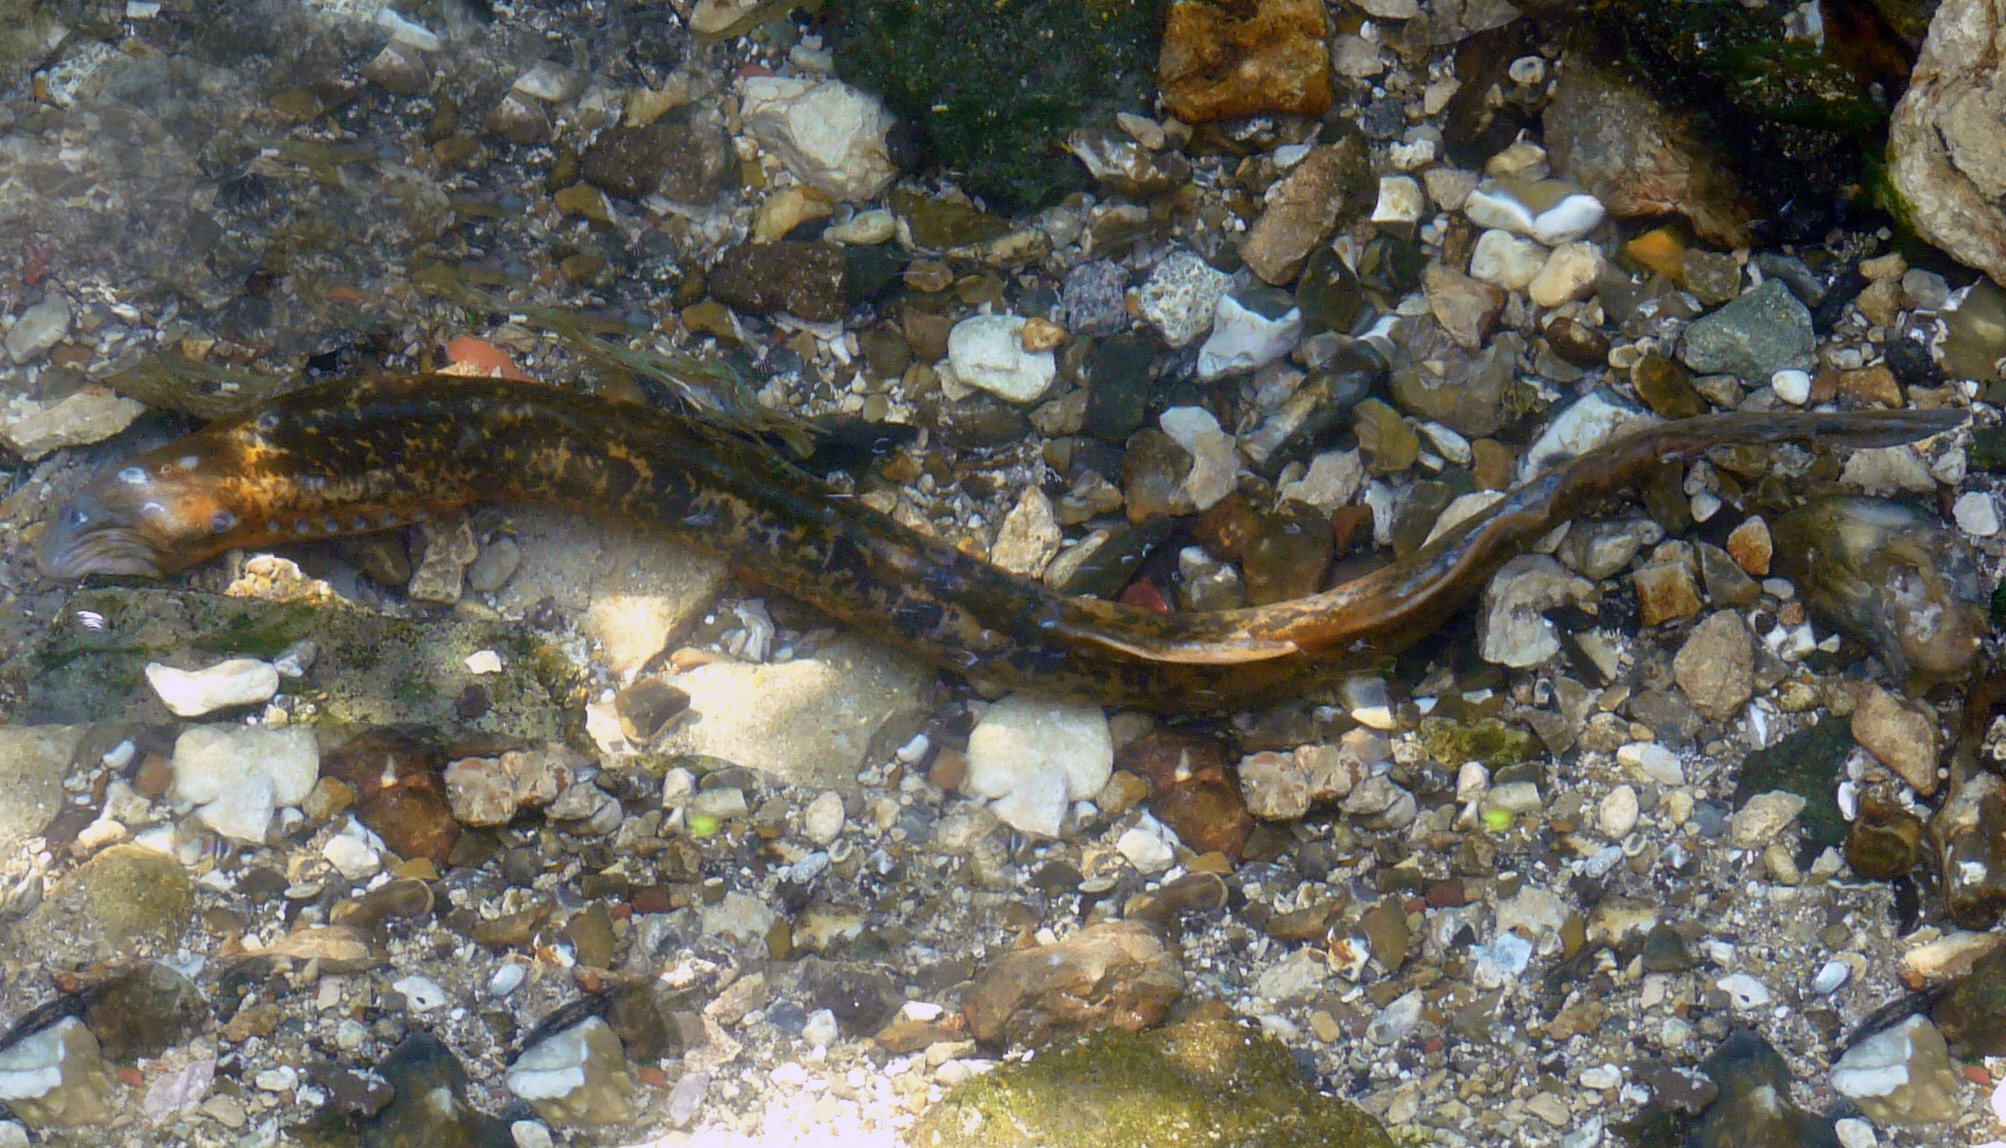
\includegraphics[width=\textwidth]{LPM_frayere}
    \end{subfigure}
       \caption{A gauche, Lamproie marine à Romilly-sur-Andelle; à droite, Lamproie marine de l'Andelle sur une frayère}
       \label{photo_lamproies}
\end{figure}

\clearpage

\section{Matériels et Méthodes}

\subsection{Site de Poses - Amfreville-sous-les-Monts}

\subsubsection{Barrage}

Le barrage de Poses représente un point stratégique dans le suivi des effectifs de migration (Figure \ref{reseau_stacomi}). Il s'agit en effet du premier ouvrage sur la Seine, à 160km de la mer et situe donc le premier point de passage obligatoire pour les migrateurs qui vont se disperser en amont, sur les 65 000 km$^2$ du bassin versant (de la Seine continentale). La présence d'une station de contrôle des migrations sur cet ouvrage, permet aujourd'hui d'identifier et de quantifier les poissons grands migrateurs en montaison chaque année sur l'axe Seine, à l'exception des géniteurs qui trouvent chaque année des zones propices à leur reproduction sur les affluents estuariens cités précédemment.

Le barrage fut construit en 1885 sur un seuil naturel à des fins de navigation entre les communes de Poses et d'Amfreville-sous-les-Monts (Eure) (Figure \ref{vue_aerienne_poses}). Il fixe la limite de marée dynamique, séparant donc, l'estuaire en aval, de la Seine continentale en amont. Long de 470 mètres, de berge à berge, et présentant une hauteur de chute de 5,4 mètres, l'ensemble de l'ouvrage se décompose en 3 parties : les écluses gérées par Voies Navigables de France (VNF) en rive droite, les vannes sur une distance de 235 mètres, et l'usine hydroélectrique gérée par HYDROWATT en rive gauche.

\begin{figure}[htpb]
\centering
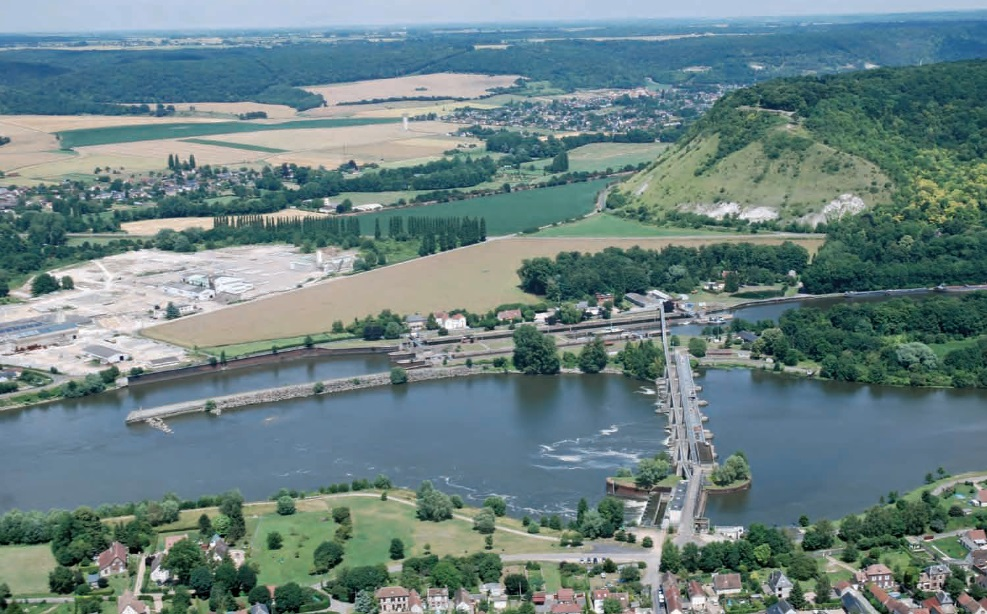
\includegraphics[width=0.8\textwidth]{vue_aerienne_poses}
\caption{Vue aérienne du barrage et des écluses de Poses - Amfreville-sous-les-Monts}
\label{vue_aerienne_poses}
\end{figure}

\subsubsection{Dispositif de franchissement}

A la construction de l'usine hydroélectrique en 1991, une passe à poissons a été construite afin de la mettre en conformité vis-à-vis de son installation sur la Seine (Figure \ref{DF_rg_poses}). En effet, au titre de la loi sur l'eau du 16 décembre 1964, tous les ouvrages doivent satisfaire les exigences de libre circulation piscicole dans les cours d'eaux classés, dont la Seine fait partie. Ce classement a été réformé et est aujourd'hui encadré par la Loi sur l'Eau et les Milieux Aquatiques (LEMA).

La passe est de type passe à bassins à fentes verticales, elle est composée d'un by-pass de dévalaison et de 23 bassins qui s'enchaînent sur une longueur de 86 mètres. En 2013, un dispositif spécifique pour le franchissement des anguilles a été construit (Figure \ref{DF_rg_poses}). Il se découpe en 3 parties; un système aval constitué de 3 rampes de type \og tapis-brosse \fg{} séparées par des bassins de repos, les anguilles sont alors dirigés vers le deuxième système qui consiste en un canal de liaison d'une longueur de 56 m avec une pente négative (2\%) débouchant sur la dernière partie de la passe, qui est un dispositif de piégeage.

\begin{figure}
\centering
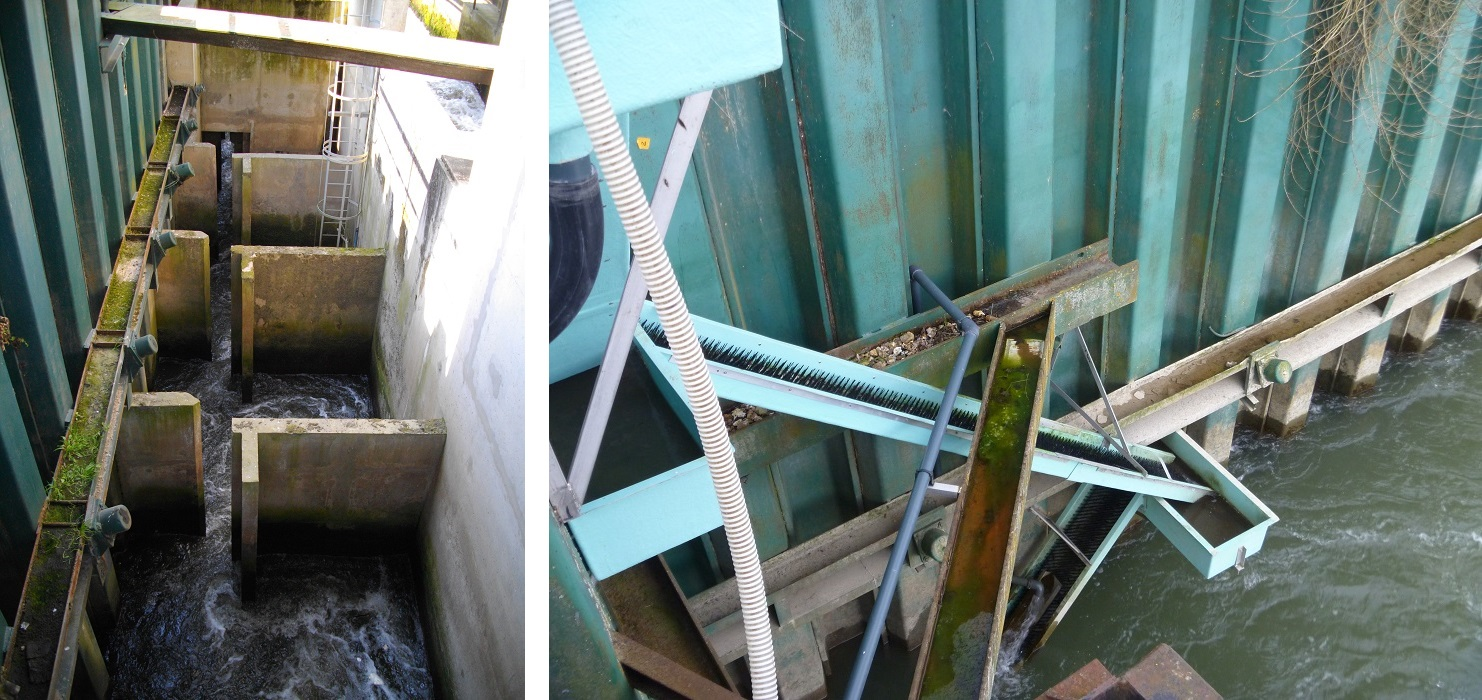
\includegraphics[width=0.8\textwidth]{DF_rg_poses}
\caption{Dispositif de franchissement en rive gauche du barrage de Poses - Amfreville-sous-les-Monts. A gauche, passe à bassins à fentes verticales; à droite, rampes de types \og tapis-brosse \fg{}}
\label{DF_rg_poses}
\end{figure}

\begin{figure}
\centering
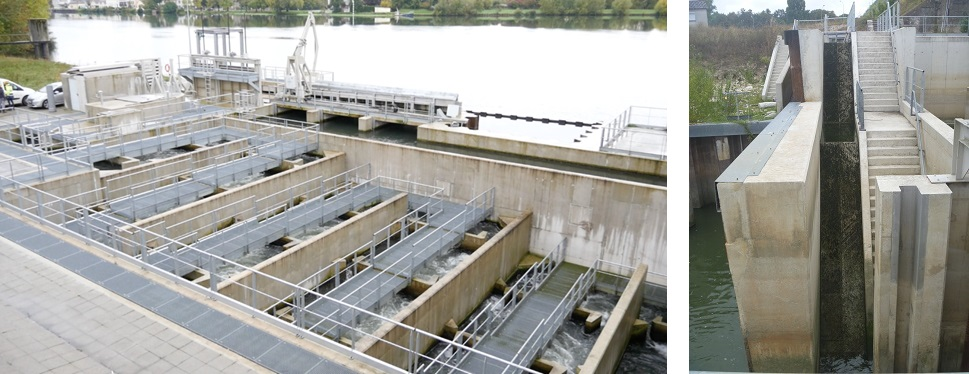
\includegraphics[width=0.8\textwidth]{DF_rd_poses}
\caption{Dispositif de franchissement en rive droite du barrage de Poses - Amfreville-sous-les-Monts. A gauche, passe à bassins à fentes verticales; à droite, rampes de types \og tapis-brosse \fg{}}
\label{DF_rd_poses}
\end{figure}

En raison de la largeur de la Seine, VNF a construit un deuxième dispositif de franchissement piscicole en rive droite (Figure \ref{DF_rd_poses}) qui vient compléter celui présent au niveau de l'usine hydroélectrique. Cet aménagement est fonctionnel depuis 2017.
Ce dispositif se compose d'une passe à poissons et d'une passe à anguilles permettant d'assurer la libre circulation pour l'ensemble des poissons. La passe à poissons est également de type passe à bassins à fentes verticales. Elle est constituée de 28 bassins qui s'enchaînent sur une longueur de 60 mètres et une largeur de 28 mètres. La passe à anguilles est constituée en partie aval de deux rampes successives de type \og tapis-brosse \fg{}, séparée par un bassin de repos, amenant à un canal longeant la passe à poissons sur une centaine de mètres et débouchant sur un dispositif de piégeage (Figure \ref{schema_passes}).


\begin{figure}[hptb]
    \centering
    \begin{subfigure}[b]{0.40\textwidth}
        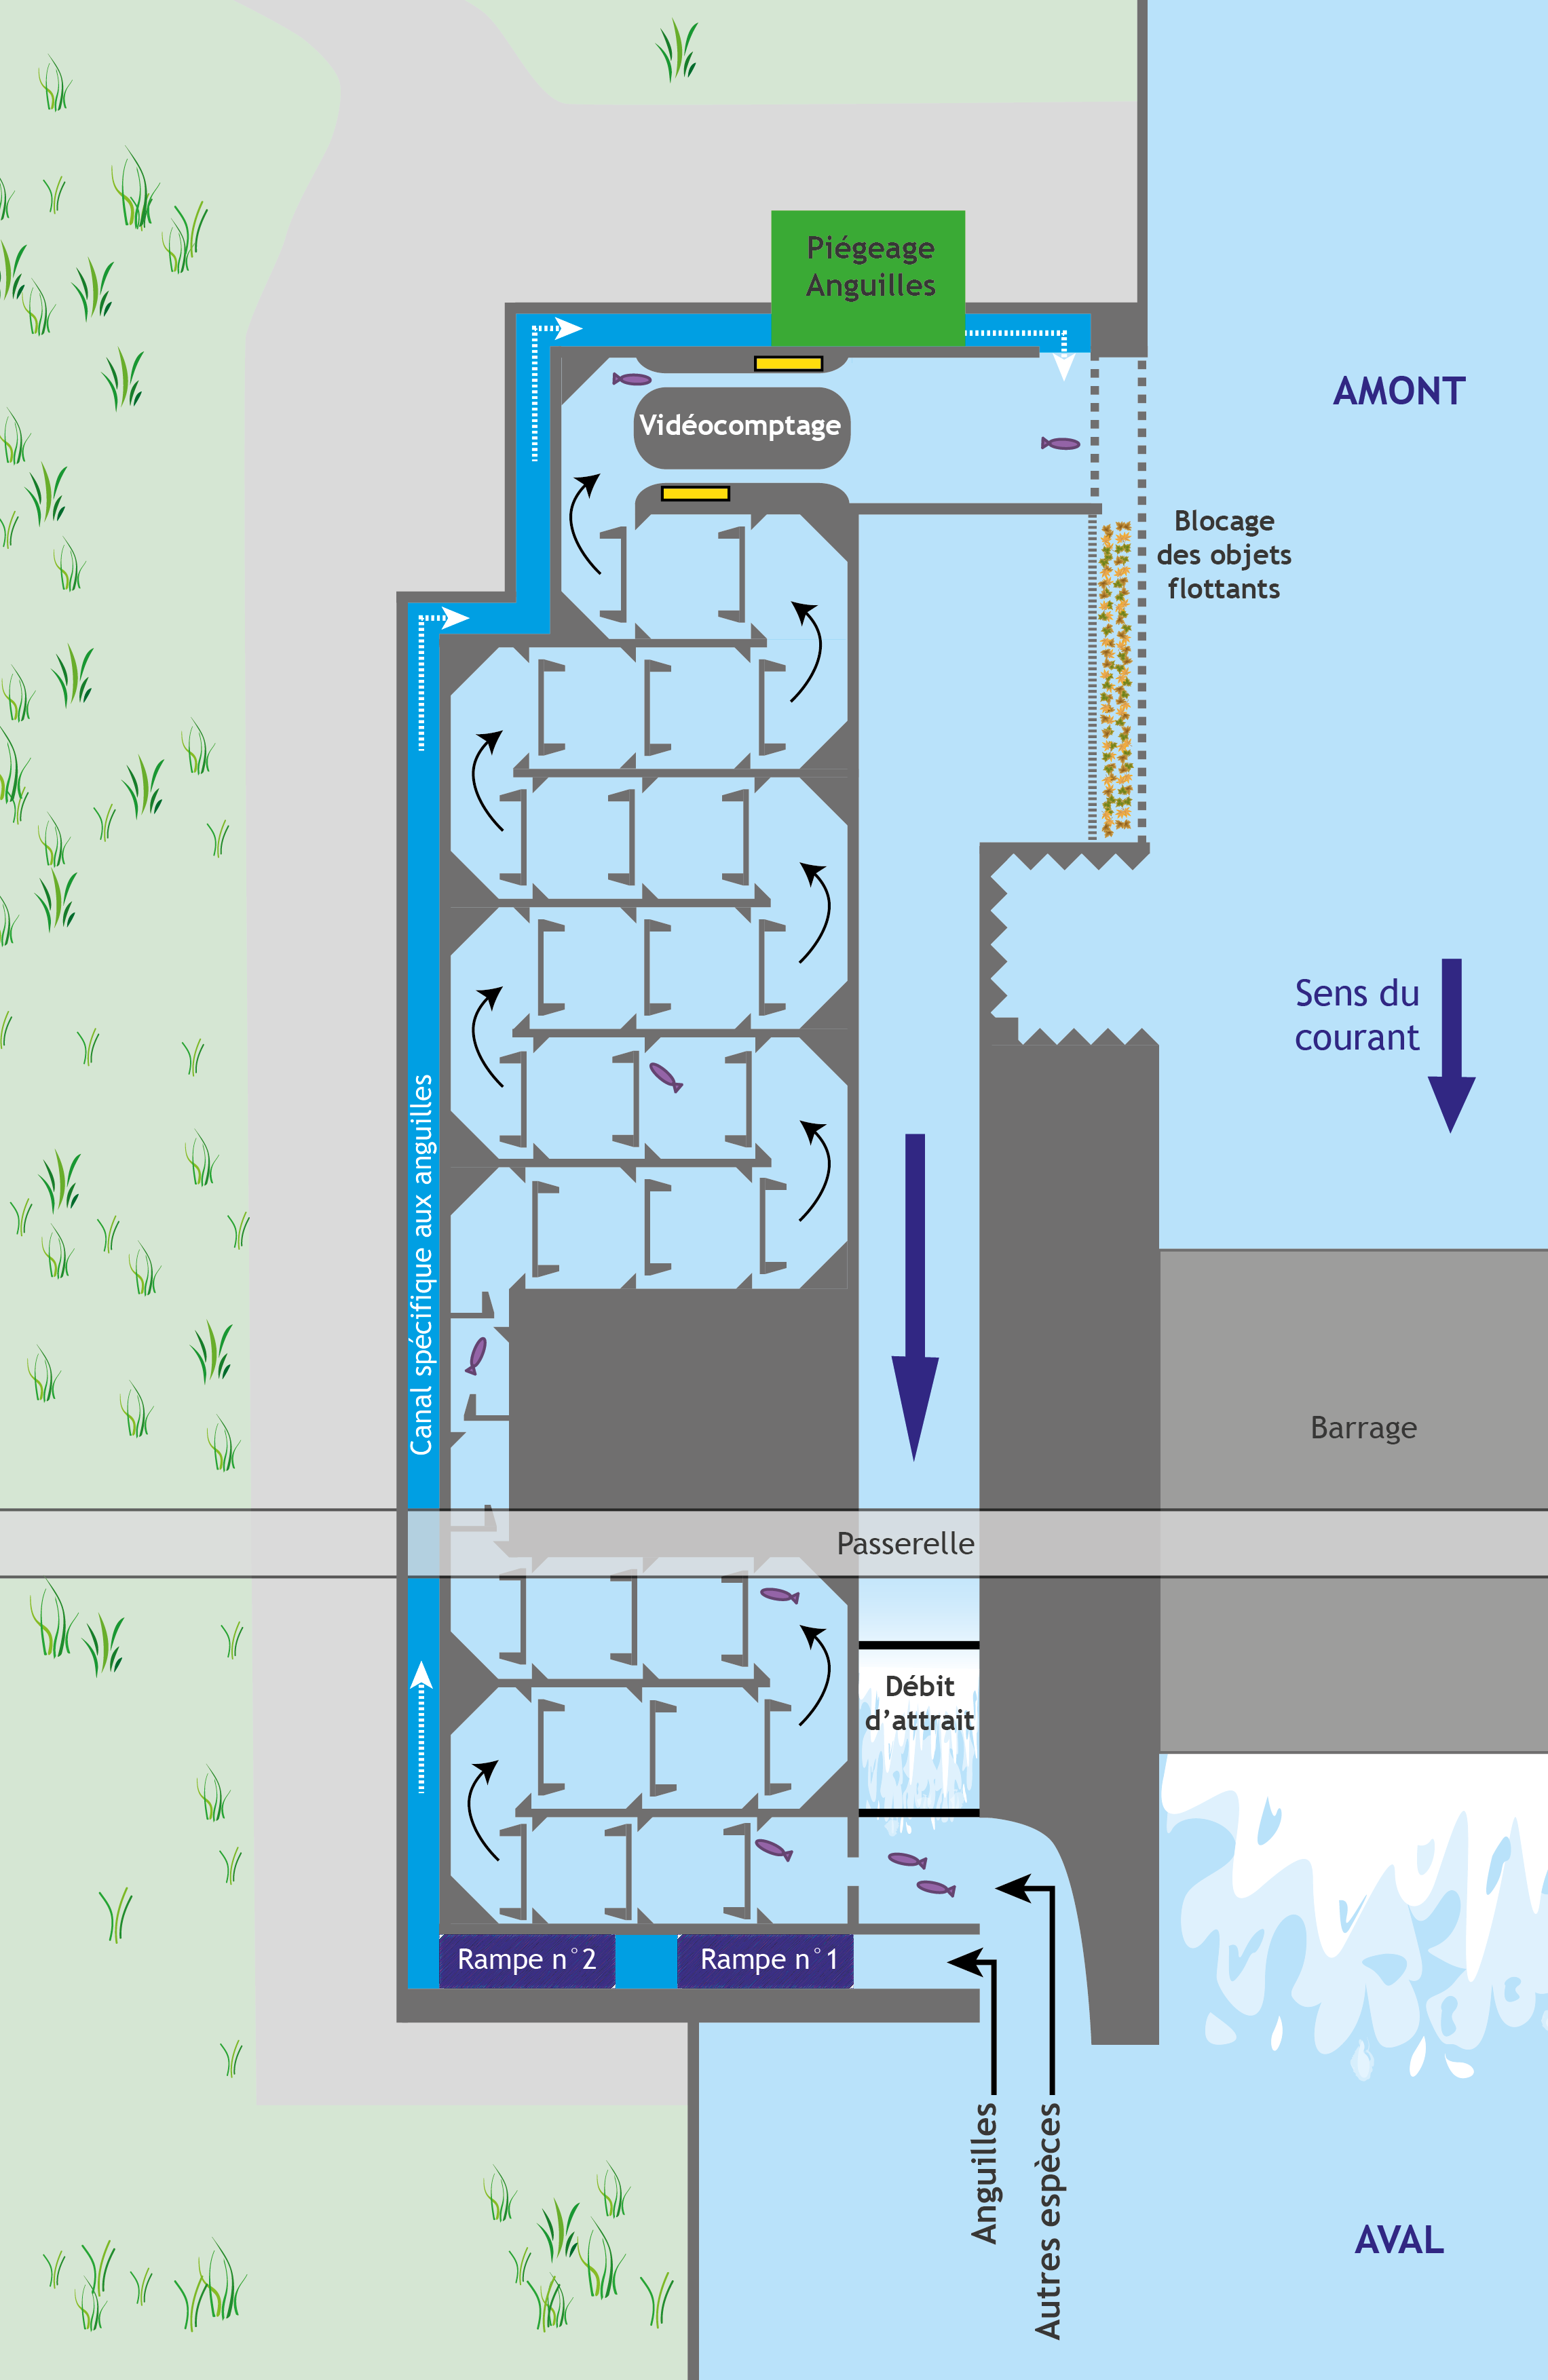
\includegraphics[width=\textwidth]{schema_passe_rd_poses}
    \end{subfigure}
    \begin{subfigure}[b]{0.448\textwidth}
        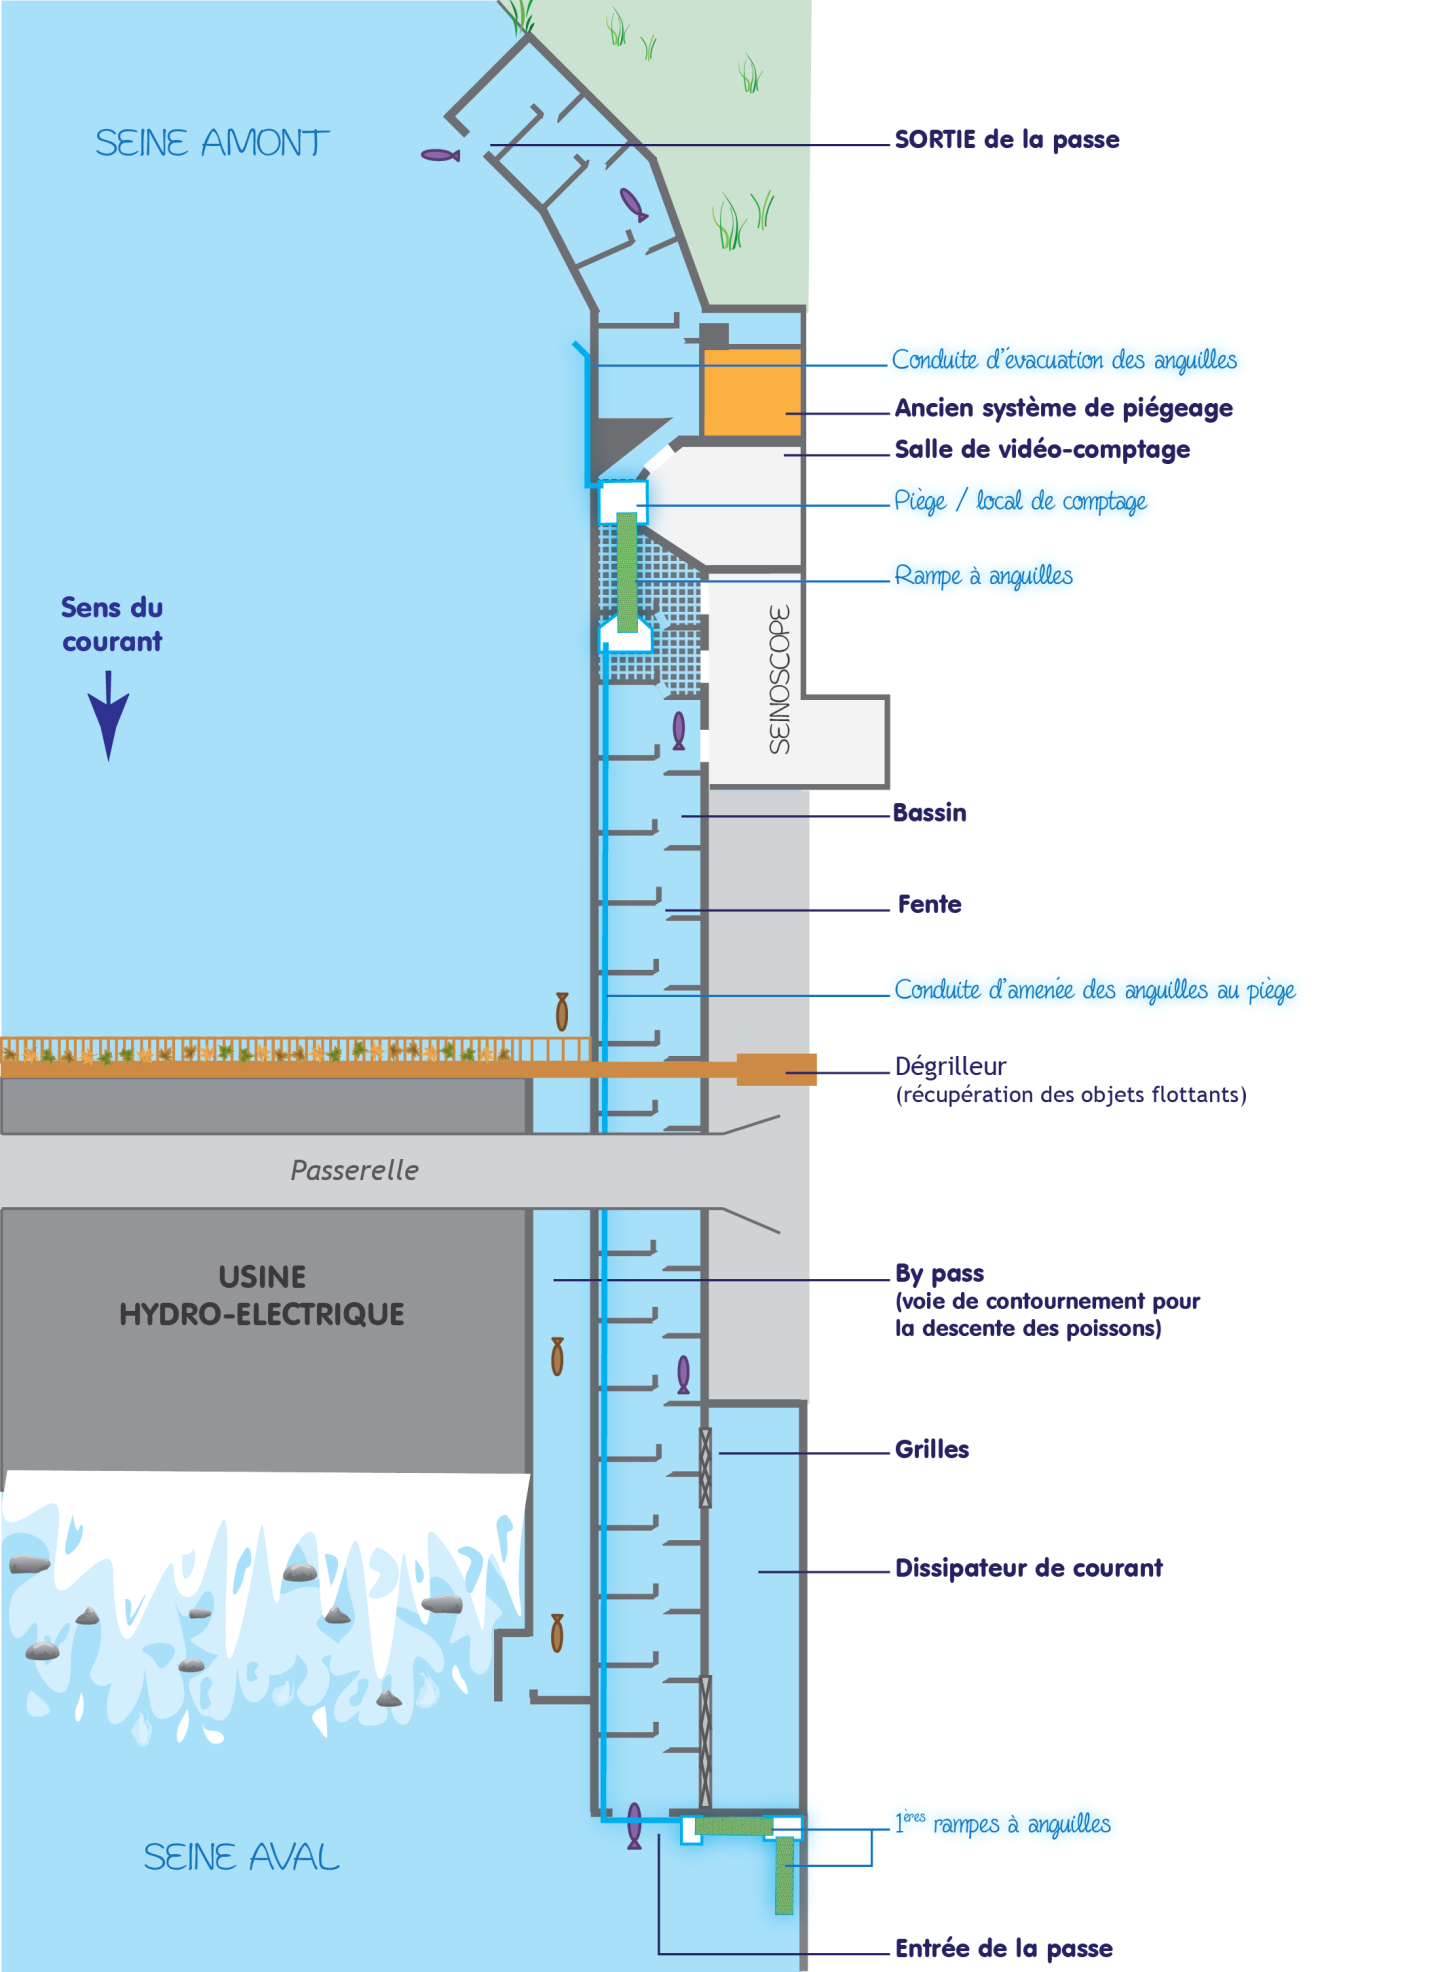
\includegraphics[width=\textwidth]{schema_passe_rg_poses}
    \end{subfigure}
       \caption{A gauche, schéma de la passe à poissons en rive droite du barrage de Poses - Amfreville-sous-les-Monts; à droite, schéma de la passe à poissons en rive gauche du barrage de Poses - Amfreville-sous-les-Monts}
       \label{schema_passes}
\end{figure}

\subsection{Site de Pontoise}

\subsubsection{Barrage}

L’ouvrage situé sur l’Oise, entre les communes de Pontoise et de Saint-Ouen l’Aumône place le dispositif de franchissement et de contrôle à 14 kilomètres de la confluence avec la Seine et à 293 km de la mer. Constitué de deux vannes, avec pour usage principal la navigation, la hauteur de chute générée par l’obstacle est de l’ordre de 1,5 mètre. Propriété de VNF (Voies Navigables de France) son usage a nécessité la construction d’un dispositif de franchissement d’envergure adapté au gabarit de la rivière.

\subsubsection{Dispositif de franchissement}

La passe à poissons a été aménagée en rive gauche sur le bras droit de la rivière en opposition avec les écluses
de navigation. Composée d’une série de huit bassins à fentes verticales permettant la remontée d’une majorité
d’espèces de poissons, une vitre d’observation est en place et a permis l'installation d'un système de vidéo-
comptage en avril 2023. Il permet d' enregistrer les remontées sur cet affluent majeur de la Seine et statuer en partie sur le
devenir des individus contrôlés en sortie d’estuaire à Poses- Amfreville-sous-les-Monts.

\subsection{Site de Carandeau}

\subsubsection{Barrage}

Le barrage de Carandeau est située sur l'Aisne au niveau de la commune de Choisy-au-Bac dans le département de l’Oise, à seulement 2 km de sa confluence avec l’Oise et à 390 km de la mer. Cet ouvrage a fait l'objet d'une modernisation dans le cadre d'un partenariat signé en 2013 entre Voies navigables de France (VNF) et la société BAMEO permettant l'automatisation de la gestion du barrage et la restauration de la continuité écologique par l'ajout d'un dispositif de franchissement piscicole.

\subsubsection{Dispositif de franchissement}

La passe à poissons est située sur la rive droite et est constituée de 8 bassins successifs à fentes verticales qui se termine par deux couloirs de comptage. Sa construction a été terminée au cours de l'année 2017 et l'installation du système de comptage a été immédiate. Les obstacles entre la mer et l’aval de l’ouvrage sont tous équipés et théoriquement franchissables. Les informations qu’apportent cette station sont donc très importantes pour évaluer l’efficacité des nouveaux dispositifs à l’aval et pour estimer la recolonisation récente du bassin de l’Aisne par les amphihalins.

\subsection{Contrôle des migrations}

Le suivi des migrations est réalisé conjointement par l'association Seinormigr et par le syndicat mixte de la Base de Plein Air et de Loisirs de Léry-Poses.
L'association Seinormigr contrôle les migrations à partir de trois dispositifs de contrôle, deux systèmes de piégeage spécifique pour les anguilles de chaque côté du fleuve ainsi qu'un système de vidéo-comptage en rive droite. Le syndicat mixte de Léry-Poses en Normandie gère le système de vidéo-comptage en rive gauche de la Seine.
Cette année, l'association a pris en charge au cours de l'année le suivi du système vidéo en rive gauche et l'intégralité de son dépouillement qui n'était plus assuré par le syndicat suite à un problème de personnel.
Différents paramètres environnementaux (débit, température, coefficient de marée...) sont relevés afin d'établir des corrélations avec les cinétiques migratoires des poissons.

\subsubsection{Dispositif de vidéo-comptage}

Afin de permettre le suivi des migrations piscicoles au niveau des passes à bassins, des dispositifs de contrôle sous forme d'un vidéo-comptage et d'un enregistrement informatique à déclenchement automatique sont en service depuis l'année 2008 en rive gauche et depuis l'automne 2017 en rive droite (Figure \ref{chambre_vc_poses}). Ce type de comptage numérique est une technique de comptage en continu sans manipulation des poissons qui permet un dénombrement en s'affranchissant des inconvénients majeurs du piégeage. Il consiste à faire passer les poissons dans une zone où ils sont suffisamment visibles pour être identifiables et dénombrables à chacun de leur passage.

\begin{figure}
\centering
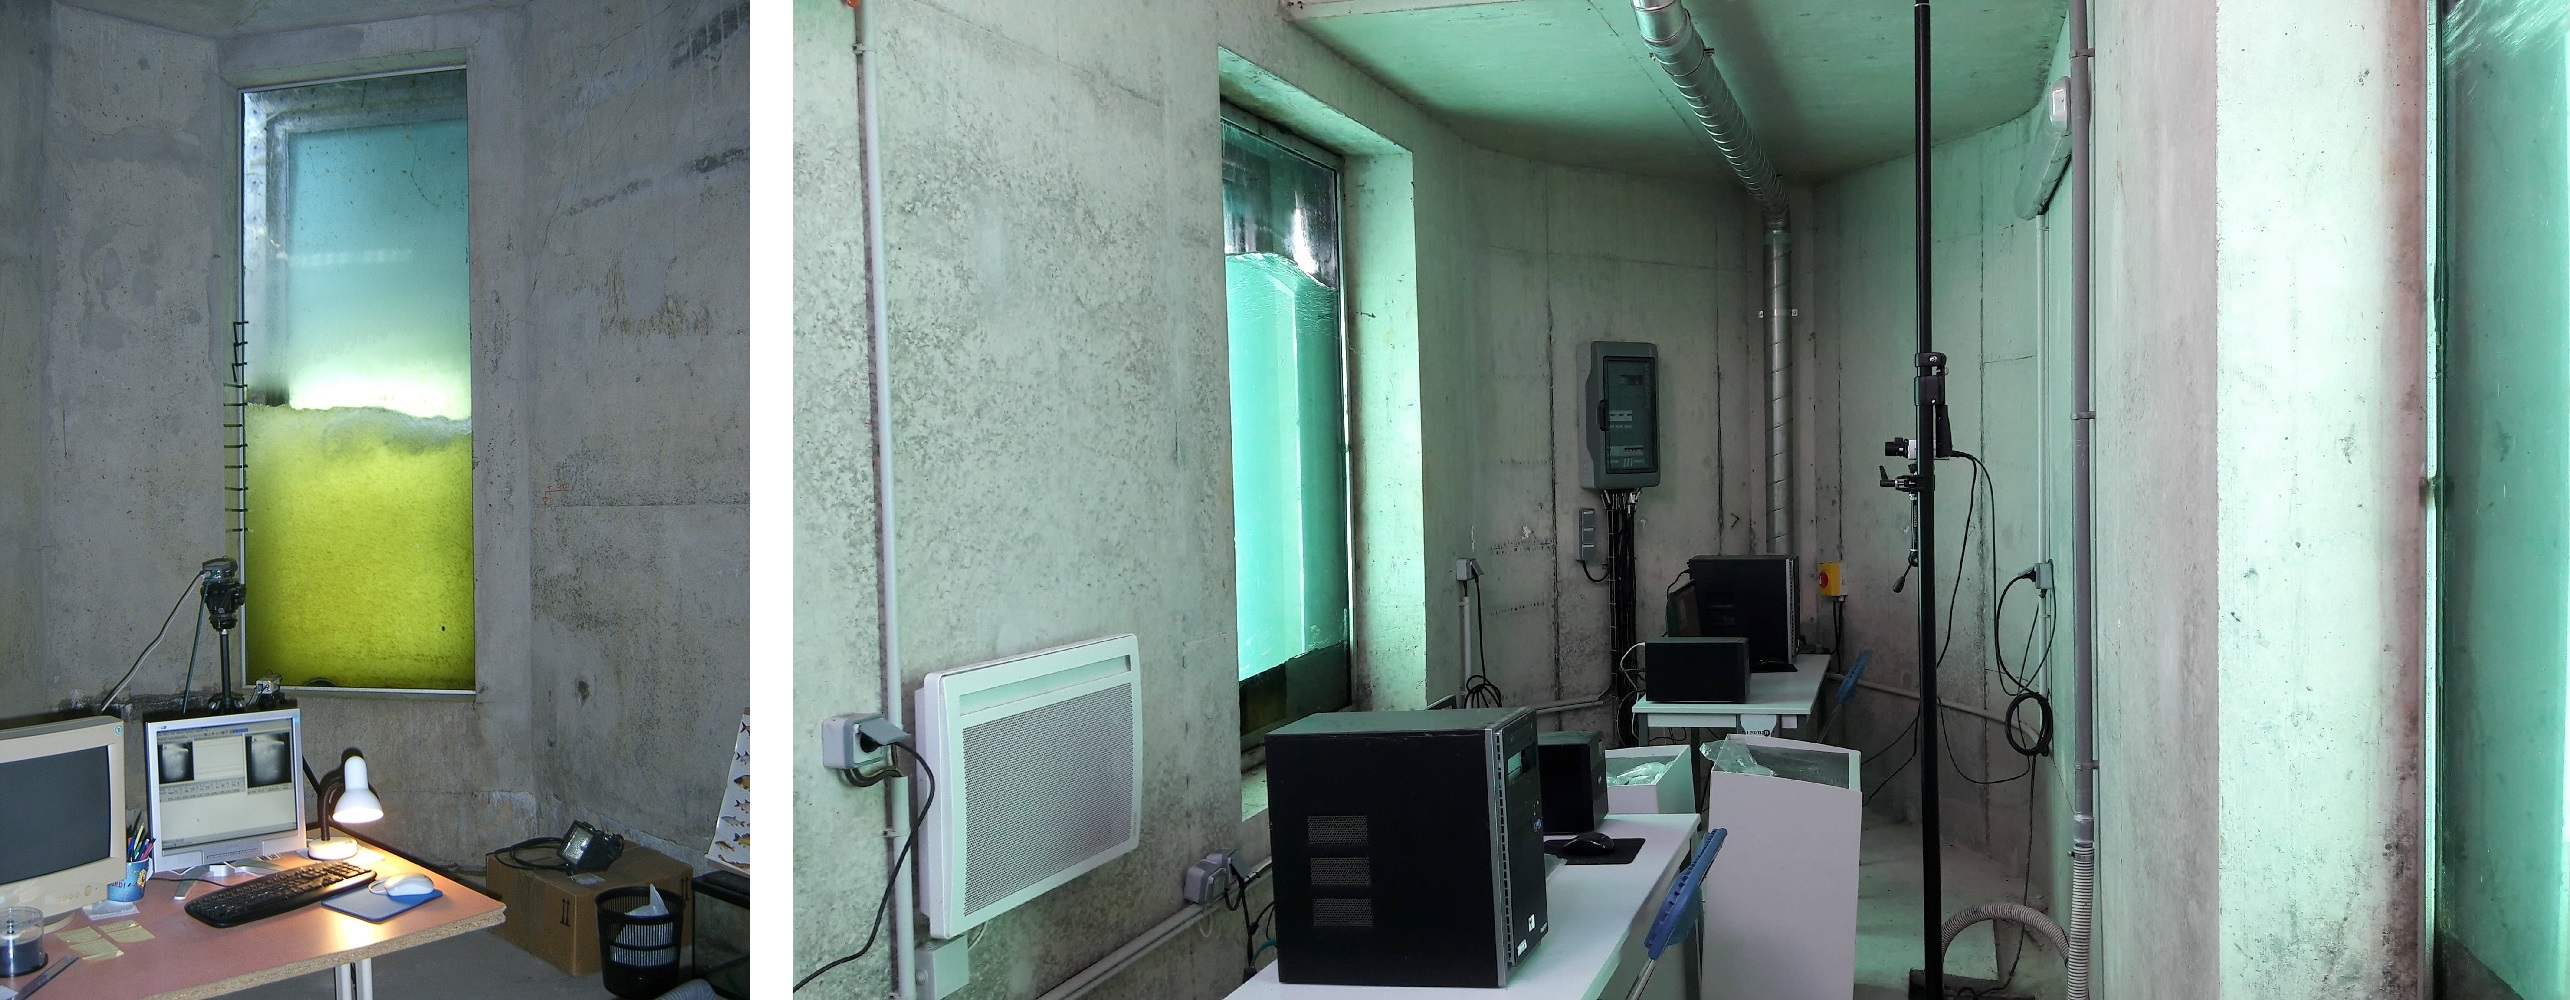
\includegraphics[width=\textwidth]{chambre_vc_poses}
\caption{Chambres de vidéo-comptage de la station de contrôle des migrations du barrage de Poses - Amfreville-sous-les-Monts. A gauche, chambre de la rive gauche; à droite, chambre de la rive droite}
\label{chambre_vc_poses}
\end{figure}

Les avantages du comptage numérique sont multiples : absence de manipulation des poissons, possibilité de comptages des espèces difficiles à piéger (aloses), charge en personnel moins lourde que pour le piégeage, précision extrême sur la détermination des rythmes migratoires et sur le comportement de l'ensemble des espèces. Les inconvénients sont l'impossibilité de comptage par forte turbidité de l'eau et la difficulté de détermination de certaines espèces (petits cyprinidés). Pour les systèmes automatisés, on se heurte également à l'efficacité partielle de détection de certaines espèces et à la sensibilité du système aux corps dérivants (herbiers en particulier) qui provoquent des déclenchements intempestifs de l'enregistrement vidéo. Dans les zones où de nombreuses espèces sont présentes une grande partie de l'année, le travail de dépouillement des données vidéo reste relativement lourd et fastidieux.

\begin{figure}
\centering
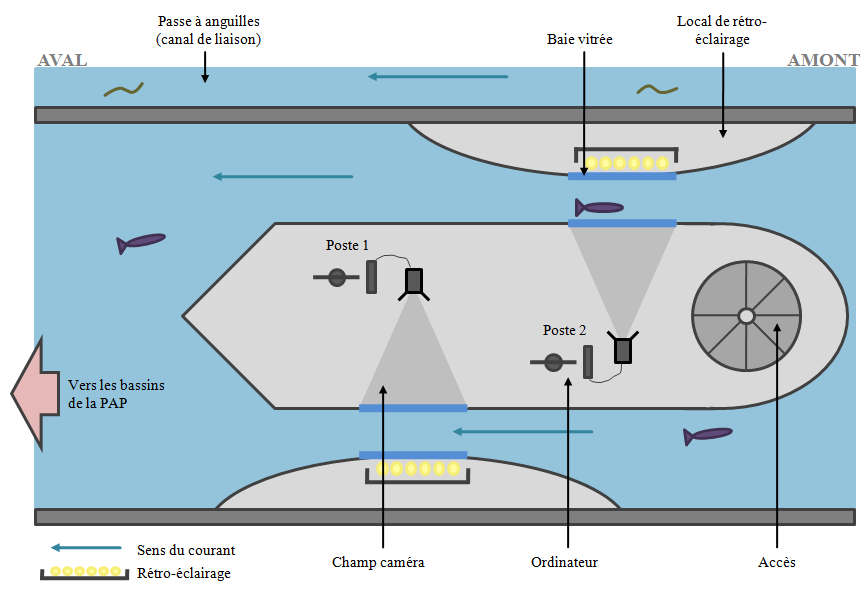
\includegraphics[width=0.8\textwidth]{vc_rd_poses}
\caption{Schéma du système de vidéo-comptage de la station de contrôle des migrations en rive droite du barrage de Poses - Amfreville-sous-les-Monts}
\label{vc_rd_poses}
\end{figure}

\begin{figure}
\centering
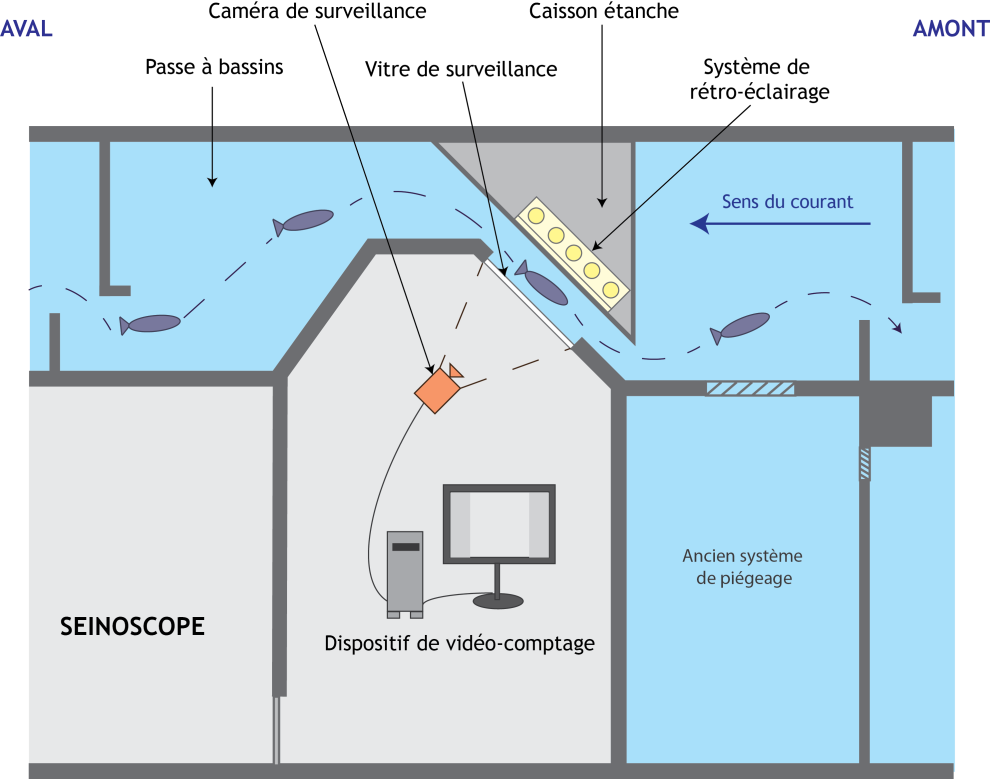
\includegraphics[width=0.8\textwidth]{vc_rg_poses}
\caption{Schéma du système de vidéo-comptage de la station de contrôle des migrations en rive gauche du barrage de Poses - Amfreville-sous-les-Monts}
\label{vc_rg_poses}
\end{figure}

Le dispositif de vidéo-comptage utilisé à la station de contrôle des migrations est basé sur le système SYSIPAP (CATTOEN, INP-ENSHEEIT) (Figure \ref{vc_rd_poses} et Figure \ref{vc_rg_poses}). Le poisson est amené à s'engager dans un couloir de vision muni de part et d'autre de deux parois vitrées, derrière lesquelles se trouvent en vis-à-vis un rétroéclairage et une caméra filmant ainsi en continu la colonne d'eau où le poisson se présentera. La passe à bassins en rive gauche est munie d'une vitre d'observation tandis que la passe de la rive droite est munie d'un double couloir de visualisation permettant de maintenir des vitesses de courant compatibles au franchissement piscicole. Il y a donc deux systèmes de comptage indépendants en rive droite. Lorsqu'un objet transite par un des couloirs de vision, celui-ci est alors détecté par un analyseur d'images qui, selon le seuil de détection qui lui a été imposé, déclenche l'enregistrement, lequel se poursuit tant qu'un objet est toujours visible et/ou détectable. Chaque séquence vidéo (10 Mo) est alors stockée dans un serveur de stockage de données informatiques prévu à cet effet. Le rôle du système de rétroéclairage disposé derrière la vitre opposée est ainsi d'accentuer le contraste afin de faciliter la détection et la reconnaissance de l'objet. Néanmoins un certain nombre de réglages doivent être appliqués, afin d'étalonner le dispositif en fonction des caractéristiques du site et des espèces de poissons présentes dans le milieu.

La fiabilité de détection du poisson devant la vitre dépend de divers paramètres de milieu (éclairage, turbidité de l'eau pour laquelle un minimum de 0,70 m au disque de Secchi est requis) et des espèces de poissons considérées (en fonction de leur taille, de leur couleur, de leur vitesse et de leur profondeur de nage). En moyenne, dans de bonnes conditions de visibilité, la fiabilité de détection est excellente (90\% à 100\%) pour les salmonidés, les aloses et les cyprinidés de taille supérieure à 25 cm, bonne (70\% à 90\%) pour les lamproies, barbeaux et cyprinidés de taille comprise entre 10 cm et 25 cm, et moyenne (50\% à 70\%) pour l'anguille et les poissons de taille inférieure à 10 cm \citep{travade_les_1992}.

Une surveillance régulière est nécessaire pour contrôler les réglages des dispositifs, nettoyer les vitres de visualisation et les zones de passage des poissons.

\subsubsection{Dépouillement des données de vidéo-comptage}

Suite à l'enregistrement des séquences vidéo, celles-ci sont récupérées par un opérateur en vue de leur dépouillement sous le logiciel WPOIS. Cette phase de dépouillement consiste en l'analyse de ces vidéos afin d'identifier et de comptabiliser les poissons traversant la passe.

Les durées de dépouillement sont très variables. En réalité ces valeurs sont fonctions des conditions de milieu (visibilité, déclenchements parasites par des corps dérivants) et surtout des espèces comptabilisées (facilité de distinction des espèces, vitesse de passage, passages isolés ou en bancs, allers et retours, stabulation devant la vitre). A l'expérience des comptages \textit{in situ}, il ressort qu'en moyenne les durées de dépouillement sont de l'ordre de 4\% à 10\% du temps réel de surveillance (soit 1 h à 2,5 h par 24 h de suivi) pour les faibles passages (inférieurs à 400 poissons/jour) et de l'ordre de 15\% à 20\% du temps réel (soit 3,5 h à 5 h par 24 h de suivi) pour les passages nombreux (3 000 à 5 000 poissons/jour) \citep{travade_les_1992}.

Tous les poissons franchissant les passes sont dénombrés et identifiés lors du vidéo-comptage. L'identification se fait à l'espèce ou à la famille, notamment dans le cas de passages importants de cyprinidés.

A l'issue de cette phase de dépouillement, l'ensemble des données est compilé dans un fichier unique puis importé dans le logiciel stacomiR, afin d'en assurer le traitement et l'analyse (\url{http://stacomir.r-forge.r-project.org/}).

\subsubsection{Dispositif de piégeage des anguilles}

Les systèmes de piégeage sont installés sur la partie amont des dispositifs de franchissment spécifiques aux anguilles. En rive droite, il se trouve à l'amont du canal à anguilles et, en rive gauche, en amont du canal de liaison. Ils sont constitués d'une rampe à \og tapis-brosse \fg{} débouchant sur un vivier (Figure \ref{passe_ang_rd_poses}). L'alimentation de la rampe et le débit d'attrait sont fournis par une pompe. Ces système sont débrayables et sont mis en service uniquement pendant la période de migration des anguilles, du mois d'avril jusqu'à l'automne selon les températures de la Seine. En effet, les suivis réalisés sur la passe en rive gauche montrent une reprise de la migration à partir d'une température de 14$^{\circ}$C \citep{mullet_suivi_2014,lenoir_suivi_2015,flesselle_suivi_2016,sanmartin_suivi_2018}.

\begin{figure}[htpb]
\centering
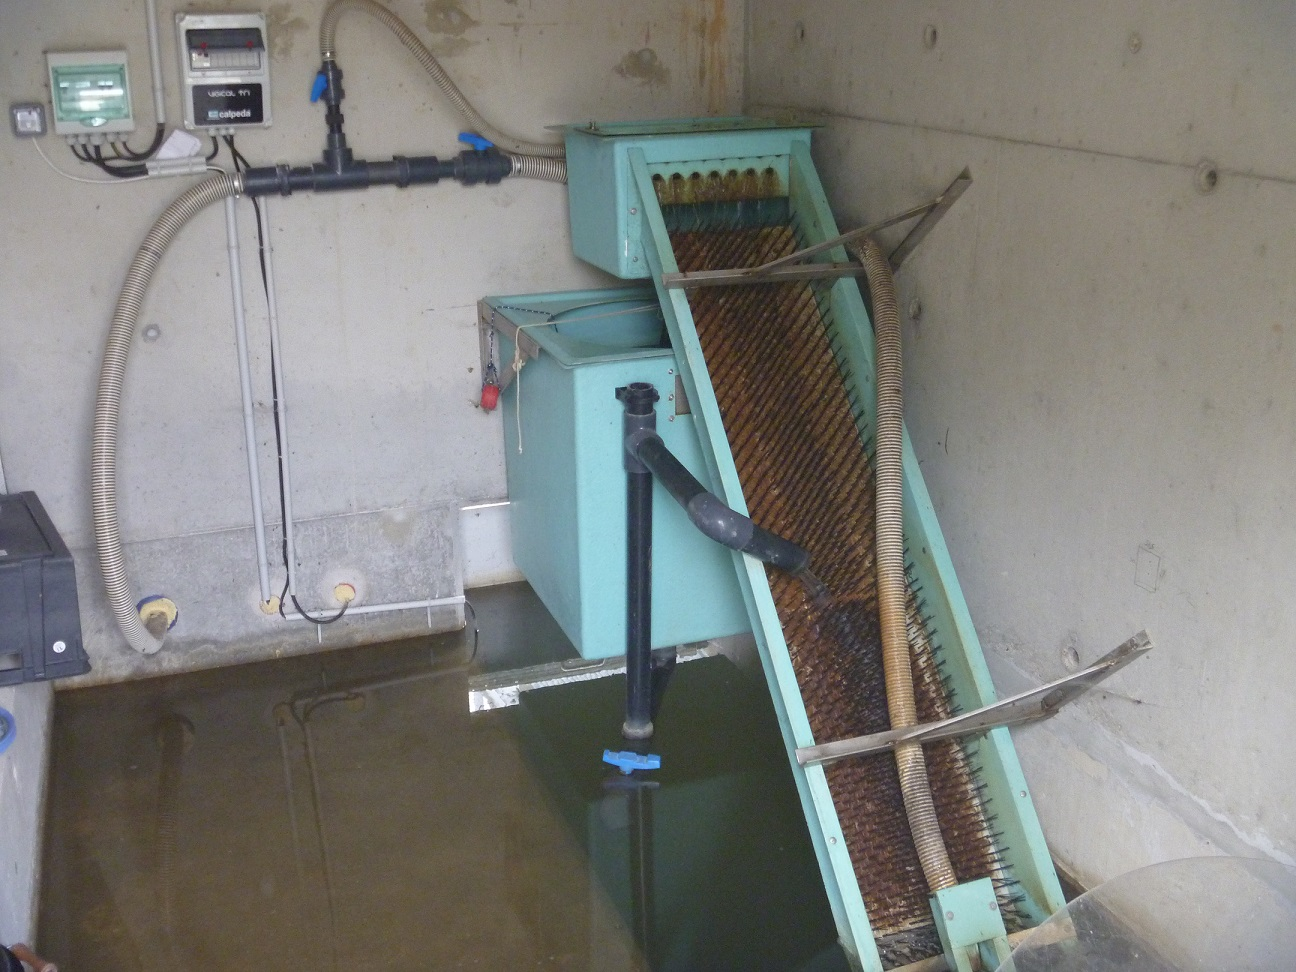
\includegraphics[width=0.8\textwidth]{passe_ang_rd_poses}
\caption{Passe piège à anguilles en rive droite du barrage de Poses - Amfreville-sous-les-Monts}
\label{passe_ang_rd_poses}
\end{figure}

\begin{figure}[htpb]
\centering
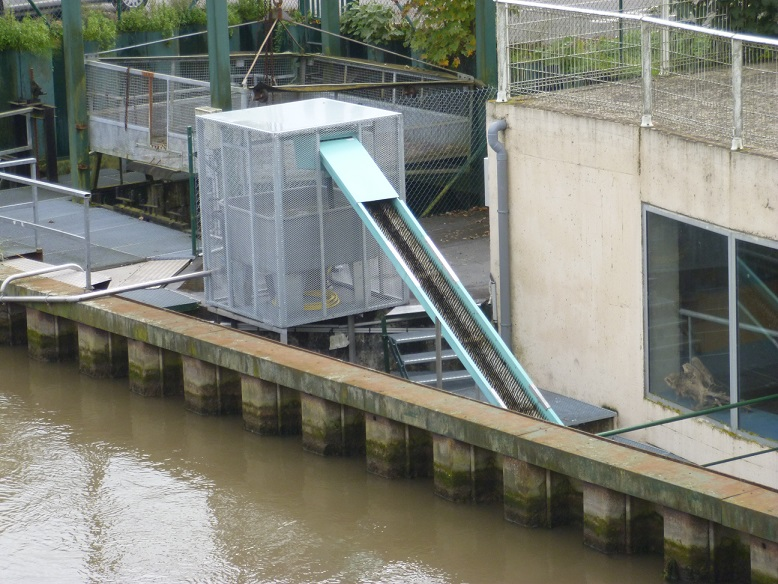
\includegraphics[width=0.8\textwidth]{passe_ang_rg_poses}
\caption{Passe piège à anguilles en rive gauche du barrage de Poses - Amfreville-sous-les-Monts}
\label{passe_ang_rg_poses}
\end{figure}

\subsubsection{Protocole de suivi}

Pendant la période de migration, le piège est relevé tous les jours, hors week-end et jours fériés excepté lors des pics de migrations. Lors de la relève du piège, la biométrie des anguilles est réalisée (Figure \ref{protocole_bio_ang}). Les individus sont préalablement anesthésiés avec une solution d'eugénol avant d'être mesurés (précision 1 mm) et pesés (précision 0,1 g). Le protocole de biométrie appliqué diffère selon la quantité d'anguilles capturées :

- Moins de 60 anguilles : biométrie individuelle

- Entre 60 et quelques milliers d'anguilles : Création de 2 lots par tamisage avec une maille de 6 mm. Pour le lot tamisé, la biométrie est effectuée sur 2 sous-lots de 30 individus et les individus restants sont pesés ensembles. Les individus du refus sont mesurés et pesés individuellement.

- Plusieurs milliers d'anguilles : Création de 3 lots de 30 individus prélevés aléatoirement, les individus des lots sont biométrés individuellement et le reste des individus est pesé globalement.

- Pic de migration exceptionnel : Un poids global est réalisé et le nombre d'anguilles est estimé en utilisant les données des suivis des jours précédents.

\begin{figure}[hptb]
    \centering
    \begin{subfigure}[b]{0.4\textwidth}
        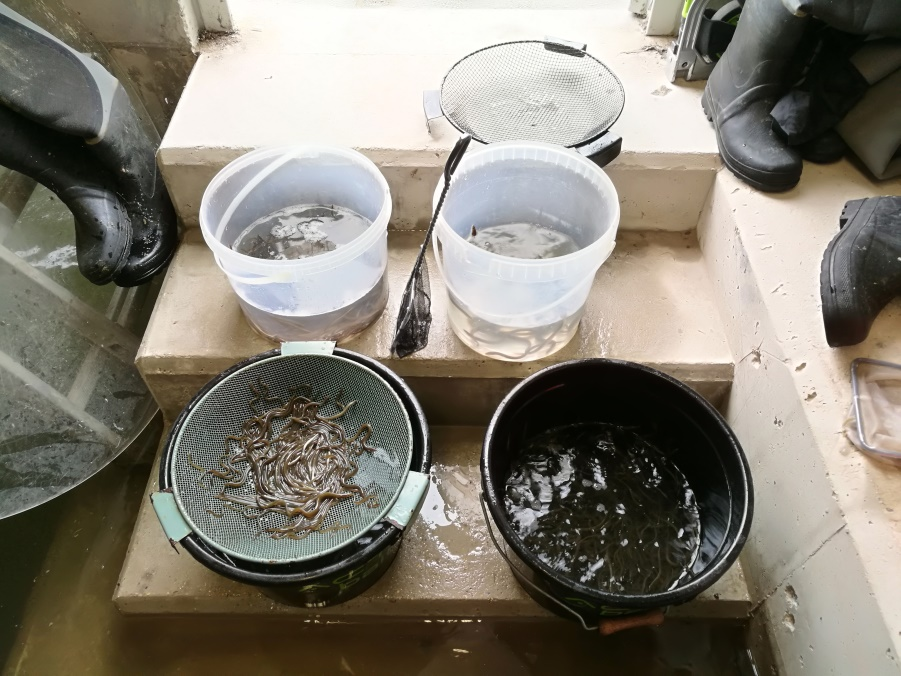
\includegraphics[width=\textwidth]{tamis_ang}
    \end{subfigure}
    \begin{subfigure}[b]{0.4\textwidth}
        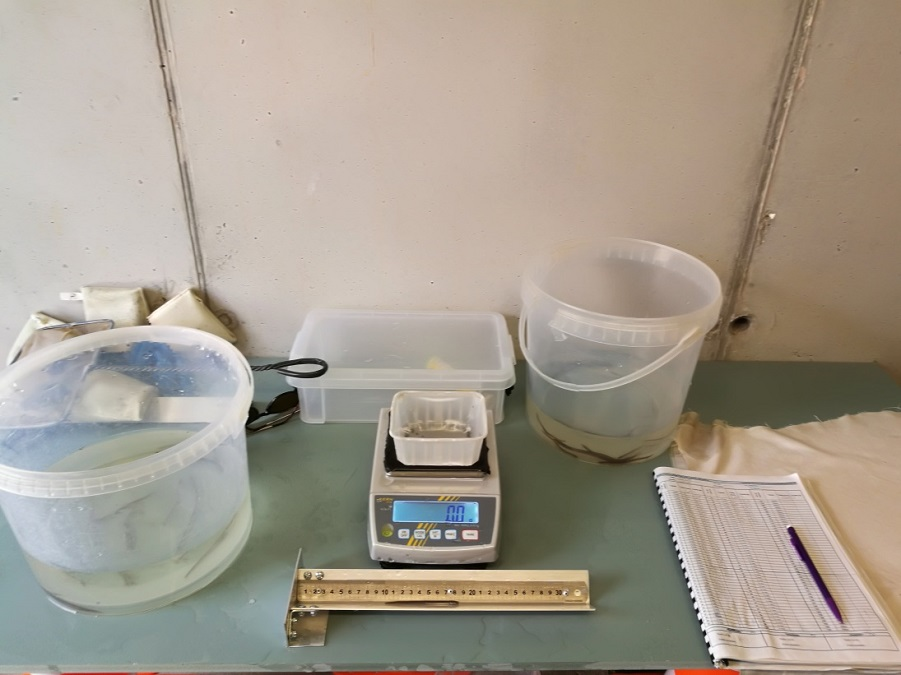
\includegraphics[width=\textwidth]{biometrie_ang}
    \end{subfigure}
       \caption{A gauche, tamisage des anguilles en différents lots de classe de taille; à droite, biométrie des anguilles capturées sur le barrage de Poses - Amfreville-sous-les-Monts}
       \label{protocole_bio_ang}
\end{figure}

\clearpage



%\twocolumn
% biblio commune aux différentes années
\bibliographystyle{apalike}
\bibliography{rapport_poses}
\normalsize
\null
\vfill

Rapport Sweave \LaTeX \\
------------------------\\
packages R : \vspace{1mm}
StacomiR \citep{legrand_stacomir_2019}\\
\LaTeX \ :Hmisc, xtable\\
graphiques : ggplot2, cowplot\\
traitements : stringr, lubridate, reshape2, dplyr, plyr, questionr\\
------------------------\\
Dernière compilation : le \today \\
 R version 4.4.1 (2024-06-14 ucrt)\\
 plateforme x86-64-w64-mingw32

\clearpage


\end{document}
